
%% bare_jrnl_compsoc.tex
%% V1.3
%% 2007/01/11
%% by Michael Shell
%% See:
%% http://www.michaelshell.org/
%% for current contact information.
%%
%% This is a skeleton file demonstrating the usef of IEEEtran.cls
%% (requires IEEEtran.cls version 1.7 or later) with an IEEE Computer
%% Society journal paper.
%%
%% Support sites:
%% http://www.michaelshell.org/tex/ieeetran/
%% http://www.ctan.org/tex-archive/macros/latex/contrib/IEEEtran/
%% and
%% http://www.ieee.org/

%%*************************************************************************
%% Legal Notice:
%% This code is offered as-is without any warranty either expressed or
%% implied; without even the implied warranty of MERCHANTABILITY or
%% FITNESS FOR A PARTICULAR PURPOSE! 
%% User assumes all risk.
%% In no event shall IEEE or any contributor to this code be liable for
%% any damages or losses, including, but not limited to, incidental,
%% consequential, or any other damages, resulting from the use or misuse
%% of any information contained here.
%%
%% All comments are the opinions of their respective authors and are not
%% necessarily endorsed by the IEEE.
%%
%% This work is distributed under the LaTeX Project Public License (LPPL)
%% ( http://www.latex-project.org/ ) version 1.3, and may be freely used,
%% distributed and modified. A copy of the LPPL, version 1.3, is included
%% in the base LaTeX documentation of all distributions of LaTeX released
%% 2003/12/01 or later.
%% Retain all contribution notices and credits.
%% ** Modified files should be clearly indicated as such, including  **
%% ** renaming them and changing author support contact information. **
%%
%% File list of work: IEEEtran.cls, IEEEtran_HOWTO.pdf, bare_adv.tex,
%%                    bare_conf.tex, bare_jrnl.tex, bare_jrnl_compsoc.tex
%%*************************************************************************

% *** Authors should verify (and, if needed, correct) their LaTeX system  ***
% *** with the testflow diagnostic prior to trusting their LaTeX platform ***
% *** with production work. IEEE's font choices can trigger bugs that do  ***
% *** not appear when using other class files.                            ***
% The testflow support page is at:
% http://www.michaelshell.org/tex/testflow/




% Note that the a4paper option is mainly intended so that authors in
% countries using A4 can easily print to A4 and see how their papers will
% look in print - the typesetting of the document will not typically be
% affected with changes in paper size (but the bottom and side margins will).
% Use the testflow package mentioned above to verify correct handling of
% both paper sizes by the user's LaTeX system.
%
% Also note that the "draftcls" or "draftclsnofoot", not "draft", option
% should be used if it is desired that the figures are to be displayed in
% draft mode.
%
% The Computer Society usually requires 10pt for submissions.
%
\documentclass[10pt,journal,cspaper,compsoc]{IEEEtran}
%
% If IEEEtran.cls has not been installed into the LaTeX system files,
% manually specify the path to it like:
% \documentclass[12pt,journal,compsoc]{../sty/IEEEtran}





% Some very useful LaTeX packages include:
% (uncomment the ones you want to load)


% *** MISC UTILITY PACKAGES ***
%
%\usepackage{ifpdf}
% Heiko Oberdiek's ifpdf.sty is very useful if you need conditional
% compilation based on whether the output is pdf or dvi.
% usage:
% \ifpdf
%   % pdf code
% \else
%   % dvi code
% \fi
% The latest version of ifpdf.sty can be obtained from:
% http://www.ctan.org/tex-archive/macros/latex/contrib/oberdiek/
% Also, note that IEEEtran.cls V1.7 and later provides a builtin
% \ifCLASSINFOpdf conditional that works the same way.
% When switching from latex to pdflatex and vice-versa, the compiler may
% have to be run twice to clear warning/error messages.


\usepackage{clrscode}
\usepackage{mathptmx}
\usepackage{graphicx}
\usepackage{times}
\usepackage{epsfig}
\usepackage{epstopdf}
\usepackage{subfig}
\usepackage{float}
\usepackage[usenames,dvipsnames]{color}

\newfloat{floatbox}{thp}{lob}[section]
\floatname{floatbox}{Algorithm}

\newcommand{\fix}[1]{{\color{red}\textbf{\textsc{[#1]}}}}


% *** CITATION PACKAGES ***
%
\ifCLASSOPTIONcompsoc
  % IEEE Computer Society needs nocompress option
  % requires cite.sty v4.0 or later (November 2003)
  % \usepackage[nocompress]{cite}
\else
  % normal IEEE
  % \usepackage{cite}
\fi
% cite.sty was written by Donald Arseneau
% V1.6 and later of IEEEtran pre-defines the format of the cite.sty package
% \cite{} output to follow that of IEEE. Loading the cite package will
% result in citation numbers being automatically sorted and properly
% "compressed/ranged". e.g., [1], [9], [2], [7], [5], [6] without using
% cite.sty will become [1], [2], [5]--[7], [9] using cite.sty. cite.sty's
% \cite will automatically add leading space, if needed. Use cite.sty's
% noadjust option (cite.sty V3.8 and later) if you want to turn this off.
% cite.sty is already installed on most LaTeX systems. Be sure and use
% version 4.0 (2003-05-27) and later if using hyperref.sty. cite.sty does
% not currently provide for hyperlinked citations.
% The latest version can be obtained at:
% http://www.ctan.org/tex-archive/macros/latex/contrib/cite/
% The documentation is contained in the cite.sty file itself.
%
% Note that some packages require special options to format as the Computer
% Society requires. In particular, Computer Society  papers do not use
% compressed citation ranges as is done in typical IEEE papers
% (e.g., [1]-[4]). Instead, they list every citation separately in order
% (e.g., [1], [2], [3], [4]). To get the latter we need to load the cite
% package with the nocompress option which is supported by cite.sty v4.0
% and later. Note also the use of a CLASSOPTION conditional provided by
% IEEEtran.cls V1.7 and later.





% *** GRAPHICS RELATED PACKAGES ***
%
\ifCLASSINFOpdf
  % \usepackage[pdftex]{graphicx}
  % declare the path(s) where your graphic files are
  % \graphicspath{{../pdf/}{../jpeg/}}
  % and their extensions so you won't have to specify these with
  % every instance of \includegraphics
  % \DeclareGraphicsExtensions{.pdf,.jpeg,.png}
\else
  % or other class option (dvipsone, dvipdf, if not using dvips). graphicx
  % will default to the driver specified in the system graphics.cfg if no
  % driver is specified.
  % \usepackage[dvips]{graphicx}
  % declare the path(s) where your graphic files are
  % \graphicspath{{../eps/}}
  % and their extensions so you won't have to specify these with
  % every instance of \includegraphics
  % \DeclareGraphicsExtensions{.eps}
\fi
% graphicx was written by David Carlisle and Sebastian Rahtz. It is
% required if you want graphics, photos, etc. graphicx.sty is already
% installed on most LaTeX systems. The latest version and documentation can
% be obtained at: 
% http://www.ctan.org/tex-archive/macros/latex/required/graphics/
% Another good source of documentation is "Using Imported Graphics in
% LaTeX2e" by Keith Reckdahl which can be found as epslatex.ps or
% epslatex.pdf at: http://www.ctan.org/tex-archive/info/
%
% latex, and pdflatex in dvi mode, support graphics in encapsulated
% postscript (.eps) format. pdflatex in pdf mode supports graphics
% in .pdf, .jpeg, .png and .mps (metapost) formats. Users should ensure
% that all non-photo figures use a vector format (.eps, .pdf, .mps) and
% not a bitmapped formats (.jpeg, .png). IEEE frowns on bitmapped formats
% which can result in "jaggedy"/blurry rendering of lines and letters as
% well as large increases in file sizes.
%
% You can find documentation about the pdfTeX application at:
% http://www.tug.org/applications/pdftex





% *** MATH PACKAGES ***
%
%\usepackage[cmex10]{amsmath}
% A popular package from the American Mathematical Society that provides
% many useful and powerful commands for dealing with mathematics. If using
% it, be sure to load this package with the cmex10 option to ensure that
% only type 1 fonts will utilized at all point sizes. Without this option,
% it is possible that some math symbols, particularly those within
% footnotes, will be rendered in bitmap form which will result in a
% document that can not be IEEE Xplore compliant!
%
% Also, note that the amsmath package sets \interdisplaylinepenalty to 10000
% thus preventing page breaks from occurring within multiline equations. Use:
%\interdisplaylinepenalty=2500
% after loading amsmath to restore such page breaks as IEEEtran.cls normally
% does. amsmath.sty is already installed on most LaTeX systems. The latest
% version and documentation can be obtained at:
% http://www.ctan.org/tex-archive/macros/latex/required/amslatex/math/





% *** SPECIALIZED LIST PACKAGES ***
%
%\usepackage{algorithmic}
% algorithmic.sty was written by Peter Williams and Rogerio Brito.
% This package provides an algorithmic environment fo describing algorithms.
% You can use the algorithmic environment in-text or within a figure
% environment to provide for a floating algorithm. Do NOT use the algorithm
% floating environment provided by algorithm.sty (by the same authors) or
% algorithm2e.sty (by Christophe Fiorio) as IEEE does not use dedicated
% algorithm float types and packages that provide these will not provide
% correct IEEE style captions. The latest version and documentation of
% algorithmic.sty can be obtained at:
% http://www.ctan.org/tex-archive/macros/latex/contrib/algorithms/
% There is also a support site at:
% http://algorithms.berlios.de/index.html
% Also of interest may be the (relatively newer and more customizable)
% algorithmicx.sty package by Szasz Janos:
% http://www.ctan.org/tex-archive/macros/latex/contrib/algorithmicx/




% *** ALIGNMENT PACKAGES ***
%
%\usepackage{array}
% Frank Mittelbach's and David Carlisle's array.sty patches and improves
% the standard LaTeX2e array and tabular environments to provide better
% appearance and additional user controls. As the default LaTeX2e table
% generation code is lacking to the point of almost being broken with
% respect to the quality of the end results, all users are strongly
% advised to use an enhanced (at the very least that provided by array.sty)
% set of table tools. array.sty is already installed on most systems. The
% latest version and documentation can be obtained at:
% http://www.ctan.org/tex-archive/macros/latex/required/tools/


%\usepackage{mdwmath}
%\usepackage{mdwtab}
% Also highly recommended is Mark Wooding's extremely powerful MDW tools,
% especially mdwmath.sty and mdwtab.sty which are used to format equations
% and tables, respectively. The MDWtools set is already installed on most
% LaTeX systems. The lastest version and documentation is available at:
% http://www.ctan.org/tex-archive/macros/latex/contrib/mdwtools/


% IEEEtran contains the IEEEeqnarray family of commands that can be used to
% generate multiline equations as well as matrices, tables, etc., of high
% quality.


%\usepackage{eqparbox}
% Also of notable interest is Scott Pakin's eqparbox package for creating
% (automatically sized) equal width boxes - aka "natural width parboxes".
% Available at:
% http://www.ctan.org/tex-archive/macros/latex/contrib/eqparbox/





% *** SUBFIGURE PACKAGES ***
%\ifCLASSOPTIONcompsoc
%\usepackage[tight,normalsize,sf,SF]{subfigure}
%\else
%\usepackage[tight,footnotesize]{subfigure}
%\fi
% subfigure.sty was written by Steven Douglas Cochran. This package makes it
% easy to put subfigures in your figures. e.g., "Figure 1a and 1b". For IEEE
% work, it is a good idea to load it with the tight package option to reduce
% the amount of white space around the subfigures. Computer Society papers
% use a larger font and \sffamily font for their captions, hence the
% additional options needed under compsoc mode. subfigure.sty is already
% installed on most LaTeX systems. The latest version and documentation can
% be obtained at:
% http://www.ctan.org/tex-archive/obsolete/macros/latex/contrib/subfigure/
% subfigure.sty has been superceeded by subfig.sty.


%\ifCLASSOPTIONcompsoc
%  \usepackage[caption=false]{caption}
%  \usepackage[font=normalsize,labelfont=sf,textfont=sf]{subfig}
%\else
%  \usepackage[caption=false]{caption}
%  \usepackage[font=footnotesize]{subfig}
%\fi
% subfig.sty, also written by Steven Douglas Cochran, is the modern
% replacement for subfigure.sty. However, subfig.sty requires and
% automatically loads Axel Sommerfeldt's caption.sty which will override
% IEEEtran.cls handling of captions and this will result in nonIEEE style
% figure/table captions. To prevent this problem, be sure and preload
% caption.sty with its "caption=false" package option. This is will preserve
% IEEEtran.cls handing of captions. Version 1.3 (2005/06/28) and later 
% (recommended due to many improvements over 1.2) of subfig.sty supports
% the caption=false option directly:
%\ifCLASSOPTIONcompsoc
%  \usepackage[caption=false,font=normalsize,labelfont=sf,textfont=sf]{subfig}
%\else
%  \usepackage[caption=false,font=footnotesize]{subfig}
%\fi
%
% The latest version and documentation can be obtained at:
% http://www.ctan.org/tex-archive/macros/latex/contrib/subfig/
% The latest version and documentation of caption.sty can be obtained at:
% http://www.ctan.org/tex-archive/macros/latex/contrib/caption/




% *** FLOAT PACKAGES ***
%
%\usepackage{fixltx2e}
% fixltx2e, the successor to the earlier fix2col.sty, was written by
% Frank Mittelbach and David Carlisle. This package corrects a few problems
% in the LaTeX2e kernel, the most notable of which is that in current
% LaTeX2e releases, the ordering of single and double column floats is not
% guaranteed to be preserved. Thus, an unpatched LaTeX2e can allow a
% single column figure to be placed prior to an earlier double column
% figure. The latest version and documentation can be found at:
% http://www.ctan.org/tex-archive/macros/latex/base/



%\usepackage{stfloats}
% stfloats.sty was written by Sigitas Tolusis. This package gives LaTeX2e
% the ability to do double column floats at the bottom of the page as well
% as the top. (e.g., "\begin{figure*}[!b]" is not normally possible in
% LaTeX2e). It also provides a command:
%\fnbelowfloat
% to enable the placement of footnotes below bottom floats (the standard
% LaTeX2e kernel puts them above bottom floats). This is an invasive package
% which rewrites many portions of the LaTeX2e float routines. It may not work
% with other packages that modify the LaTeX2e float routines. The latest
% version and documentation can be obtained at:
% http://www.ctan.org/tex-archive/macros/latex/contrib/sttools/
% Documentation is contained in the stfloats.sty comments as well as in the
% presfull.pdf file. Do not use the stfloats baselinefloat ability as IEEE
% does not allow \baselineskip to stretch. Authors submitting work to the
% IEEE should note that IEEE rarely uses double column equations and
% that authors should try to avoid such use. Do not be tempted to use the
% cuted.sty or midfloat.sty packages (also by Sigitas Tolusis) as IEEE does
% not format its papers in such ways.




%\ifCLASSOPTIONcaptionsoff
%  \usepackage[nomarkers]{endfloat}
% \let\MYoriglatexcaption\caption
% \renewcommand{\caption}[2][\relax]{\MYoriglatexcaption[#2]{#2}}
%\fi
% endfloat.sty was written by James Darrell McCauley and Jeff Goldberg.
% This package may be useful when used in conjunction with IEEEtran.cls'
% captionsoff option. Some IEEE journals/societies require that submissions
% have lists of figures/tables at the end of the paper and that
% figures/tables without any captions are placed on a page by themselves at
% the end of the document. If needed, the draftcls IEEEtran class option or
% \CLASSINPUTbaselinestretch interface can be used to increase the line
% spacing as well. Be sure and use the nomarkers option of endfloat to
% prevent endfloat from "marking" where the figures would have been placed
% in the text. The two hack lines of code above are a slight modification of
% that suggested by in the endfloat docs (section 8.3.1) to ensure that
% the full captions always appear in the list of figures/tables - even if
% the user used the short optional argument of \caption[]{}.
% IEEE papers do not typically make use of \caption[]'s optional argument,
% so this should not be an issue. A similar trick can be used to disable
% captions of packages such as subfig.sty that lack options to turn off
% the subcaptions:
% For subfig.sty:
% \let\MYorigsubfloat\subfloat
% \renewcommand{\subfloat}[2][\relax]{\MYorigsubfloat[]{#2}}
% For subfigure.sty:
% \let\MYorigsubfigure\subfigure
% \renewcommand{\subfigure}[2][\relax]{\MYorigsubfigure[]{#2}}
% However, the above trick will not work if both optional arguments of
% the \subfloat/subfig command are used. Furthermore, there needs to be a
% description of each subfigure *somewhere* and endfloat does not add
% subfigure captions to its list of figures. Thus, the best approach is to
% avoid the use of subfigure captions (many IEEE journals avoid them anyway)
% and instead reference/explain all the subfigures within the main caption.
% The latest version of endfloat.sty and its documentation can obtained at:
% http://www.ctan.org/tex-archive/macros/latex/contrib/endfloat/
%
% The IEEEtran \ifCLASSOPTIONcaptionsoff conditional can also be used
% later in the document, say, to conditionally put the References on a 
% page by themselves.




% *** PDF, URL AND HYPERLINK PACKAGES ***
%
%\usepackage{url}
% url.sty was written by Donald Arseneau. It provides better support for
% handling and breaking URLs. url.sty is already installed on most LaTeX
% systems. The latest version can be obtained at:
% http://www.ctan.org/tex-archive/macros/latex/contrib/misc/
% Read the url.sty source comments for usage information. Basically,
% \url{my_url_here}.





% *** Do not adjust lengths that control margins, column widths, etc. ***
% *** Do not use packages that alter fonts (such as pslatex).         ***
% There should be no need to do such things with IEEEtran.cls V1.6 and later.
% (Unless specifically asked to do so by the journal or conference you plan
% to submit to, of course. )


% correct bad hyphenation here
\hyphenation{op-tical net-works semi-conduc-tor}


\begin{document}
%
% paper title
% can use linebreaks \\ within to get better formatting as desired

\title{Provenance-Enabled Topological Connection Reconstruction}

%
%
% author names and IEEE memberships
% note positions of commas and nonbreaking spaces ( ~ ) LaTeX will not break
% a structure at a ~ so this keeps an author's name from being broken across
% two lines.
% use \thanks{} to gain access to the first footnote area
% a separate \thanks must be used for each paragraph as LaTeX2e's \thanks
% was not built to handle multiple paragraphs
%
%
%\IEEEcompsocitemizethanks is a special \thanks that produces the bulleted
% lists the Computer Society journals use for "first footnote" author
% affiliations. Use \IEEEcompsocthanksitem which works much like \item
% for each affiliation group. When not in compsoc mode,
% \IEEEcompsocitemizethanks becomes like \thanks and
% \IEEEcompsocthanksitem becomes a line break with idention. This
% facilitates dual compilation, although admittedly the differences in the
% desired content of \author between the different types of papers makes a
% one-size-fits-all approach a daunting prospect. For instance, compsoc 
% journal papers have the author affiliations above the "Manuscript
% received ..."  text while in non-compsoc journals this is reversed. Sigh.

\author{Robert~Miller,~\IEEEmembership{Student Member,~IEEE,}
        Kenneth~Moreland,~\IEEEmembership{Member,~IEEE,} \protect\\
        and~Kwan-Liu~Ma,~\IEEEmembership{Senior Member,~IEEE}% <-this % stops a space
\IEEEcompsocitemizethanks{\IEEEcompsocthanksitem Robert Miller and Kwan-Liu Ma are with the University of California,~Davis, 2063 Kemper Hall, One Shields Avenue, Davis, CA 95616-8562.\protect\\
% note need leading \protect in front of \\ to get a newline within \thanks as
% \\ is fragile and will error, could use \hfil\break instead.
E-mail: \{bobmiller, ma\}@ucdavis.edu
\IEEEcompsocthanksitem Kenneth Moreland is with Sandia National Labs}% <-this % stops a space
\thanks{}}

% note the % following the last \IEEEmembership and also \thanks - 
% these prevent an unwanted space from occurring between the last author name
% and the end of the author line. i.e., if you had this:
% 
% \author{....lastname \thanks{...} \thanks{...} }
%                     ^------------^------------^----Do not want these spaces!
%
% a space would be appended to the last name and could cause every name on that
% line to be shifted left slightly. This is one of those "LaTeX things". For
% instance, "\textbf{A} \textbf{B}" will typeset as "A B" not "AB". To get
% "AB" then you have to do: "\textbf{A}\textbf{B}"
% \thanks is no different in this regard, so shield the last } of each \thanks
% that ends a line with a % and do not let a space in before the next \thanks.
% Spaces after \IEEEmembership other than the last one are OK (and needed) as
% you are supposed to have spaces between the names. For what it is worth,
% this is a minor point as most people would not even notice if the said evil
% space somehow managed to creep in.



% The paper headers
%\markboth{Journal of \LaTeX\ Class Files,~Vol.~6, No.~1, January~2007}%
%{Shell \MakeLowercase{\textit{et al.}}: Bare Demo of IEEEtran.cls for Computer Society Journals}
% The only time the second header will appear is for the odd numbered pages
% after the title page when using the twoside option.
% 
% *** Note that you probably will NOT want to include the author's ***
% *** name in the headers of peer review papers.                   ***
% You can use \ifCLASSOPTIONpeerreview for conditional compilation here if
% you desire.



% The publisher's ID mark at the bottom of the page is less important with
% Computer Society journal papers as those publications place the marks
% outside of the main text columns and, therefore, unlike regular IEEE
% journals, the available text space is not reduced by their presence.
% If you want to put a publisher's ID mark on the page you can do it like
% this:
%\IEEEpubid{0000--0000/00\$00.00~\copyright~2007 IEEE}
% or like this to get the Computer Society new two part style.
%\IEEEpubid{\makebox[\columnwidth]{\hfill 0000--0000/00/\$00.00~\copyright~2007 IEEE}%
%\hspace{\columnsep}\makebox[\columnwidth]{Published by the IEEE Computer Society\hfill}}
% Remember, if you use this you must call \IEEEpubidadjcol in the second
% column for its text to clear the IEEEpubid mark (Computer Society jorunal
% papers don't need this extra clearance.)




% for Computer Society papers, we must declare the abstract and index terms
% PRIOR to the title within the \IEEEcompsoctitleabstractindextext IEEEtran
% command as these need to go into the title area created by \maketitle.
\IEEEcompsoctitleabstractindextext{%
\begin{abstract}
%\boldmath
 Many algorithms applied to mesh-based data structures are easily parallelizable because operations can often be divided by the constituent elements of the mesh and parallelized with a large number of threads. The problem with this technique is that when these threads generate new topological features, they tend to generate redundant information such as coincident vertices. This ``soup'' of elements requires significant additional memory to store and fails to capture the adjacency of neighboring elements. We present a novel approach for the efficient construction of connected topologies on multi- and many-core systems, which we demonstrate with GPU and OpenMP implementations. In this approach, we use input topological features as a basis for efficient location of coincident features in the output. We provide examples and performance numbers of the technique for isosurface generation and multiple forms of tetrahedralization.
\end{abstract}
% IEEEtran.cls defaults to using nonbold math in the Abstract.
% This preserves the distinction between vectors and scalars. However,
% if the journal you are submitting to favors bold math in the abstract,
% then you can use LaTeX's standard command \boldmath at the very start
% of the abstract to achieve this. Many IEEE journals frown on math
% in the abstract anyway. In particular, the Computer Society does
% not want either math or citations to appear in the abstract.

% Note that keywords are not normally used for peer review papers.
\begin{keywords}
Parallel Systems, GPUs and Multi-core Architectures, CPU and GPU clusters, Petascale Techniques, Scalability Issues
\end{keywords}}


% make the title area
\maketitle


% To allow for easy dual compilation without having to reenter the
% abstract/keywords data, the \IEEEcompsoctitleabstractindextext text will
% not be used in maketitle, but will appear (i.e., to be "transported")
% here as \IEEEdisplaynotcompsoctitleabstractindextext when compsoc mode
% is not selected <OR> if conference mode is selected - because compsoc
% conference papers position the abstract like regular (non-compsoc)
% papers do!
\IEEEdisplaynotcompsoctitleabstractindextext
% \IEEEdisplaynotcompsoctitleabstractindextext has no effect when using
% compsoc under a non-conference mode.


% For peer review papers, you can put extra information on the cover
% page as needed:
% \ifCLASSOPTIONpeerreview
% \begin{center} \bfseries EDICS Category: 3-BBND \end{center}
% \fi
%
% For peerreview papers, this IEEEtran command inserts a page break and
% creates the second title. It will be ignored for other modes.
\IEEEpeerreviewmaketitle



\section{Introduction}
% Computer Society journal papers do something a tad strange with the very
% first section heading (almost always called "Introduction"). They place it
% ABOVE the main text! IEEEtran.cls currently does not do this for you.
% However, You can achieve this effect by making LaTeX jump through some
% hoops via something like:
%
%\ifCLASSOPTIONcompsoc
%  \noindent\raisebox{2\baselineskip}[0pt][0pt]%
%  {\parbox{\columnwidth}{\section{Introduction}\label{sec:introduction}%
%  \global\everypar=\everypar}}%
%  \vspace{-1\baselineskip}\vspace{-\parskip}\par
%\else
%  \section{Introduction}\label{sec:introduction}\par
%\fi
%
% Admittedly, this is a hack and may well be fragile, but seems to do the
% trick for me. Note the need to keep any \label that may be used right
% after \section in the above as the hack puts \section within a raised box.



% The very first letter is a 2 line initial drop letter followed
% by the rest of the first word in caps (small caps for compsoc).
% 
% form to use if the first word consists of a single letter:
% \IEEEPARstart{A}{demo} file is ....
% 
% form to use if you need the single drop letter followed by
% normal text (unknown if ever used by IEEE):
% \IEEEPARstart{A}{}demo file is ....
% 
% Some journals put the first two words in caps:
% \IEEEPARstart{T}{his demo} file is ....
% 
% Here we have the typical use of a "T" for an initial drop letter
% and "HIS" in caps to complete the first word.
\IEEEPARstart{M}{any} existing parallel graphics techniques are designed to generate geometry from
some form of input mesh. Such algorithms tend to have the attribute that
computation of any given output feature depends solely on a small set
of input features. This provides a natural partitioning of the input
which can then be used to develop parallel algorithms. As an example,
the Marching Cubes \cite{Lorensen1987} algorithm can be parallelized per voxel, so that only
the data values at the voxel corners are necessary to generate the geometry
within the voxel (if any).

The problem with this naive parallelization is that it generates a
`soup' of output primitives, with no information about connectivity.
The aforementioned Marching Cubes algorithm simply produces a set of disconnected triangles.
This is not a concern so long as all further computation on the output
depends exclusively on the local attributes of individual primitives, such as is
the case with rendering. 

Rendering has often been the ultimate goal for the
generated output of parallel graphics algorithms and the size of the output is not a concern, so these techniques have been sufficient. When
additional processing of the output is desired that requires information about the connectivity 
between multiple primitives, the situation becomes more difficult. Consider the calculation of 
the curvature of the isosurface generated by Marching Cubes.
Given only a triangle soup, there is no simple method to determine the neighbors of any given triangle, which is a required step to 
compute the curvature. A more complex example would be the case of a visualization pipeline,
where different types of topological connectivity information may be necessary depending
on the structure of the pipeline.

This is not a new problem, and techniques exist to determine topological
information about a primitive soup \cite{Park}. Generally this approach starts by finding 
and coalescing duplicate vertices, which may require a bounded-radius nearest-neighbor search to 
resolve vertices that are identical save for floating point error. Next, the algorithm finds all primitives that 
share two or more vertices, and links them together as neighbors. Finally,
some `duplicate' vertices may not actually represent desirable connections,
such as is the case where two cones meet at their apices, so these vertices
may need to be split in a final pass. This process is computationally complex, and is
specific to the topological connections between triangles. 

We present a technique which applies equally well to other types of topological 
connections, such as determining the neighboring facets of tetrahedra. Our technique makes use of the fact that geometry is rarely generated in a vacuum; we usually have some information about how the geometry is generated. To list a few examples: Marching Cubes generates its output vertices on the edges of a structured grid, dual meshes generate their vertices on the faces of an input mesh, and tetrahedralizations can be generated on an existing spatial grid or mesh. 

We explore the advantages of making a small modification to the algorithms that generate the geometry, where the information is stored about what feature of the input topology was used to generate each output feature. 

\begin{figure*}[!tb]
\subfloat[Marching Cubes\label{fig:teaser:mc}]{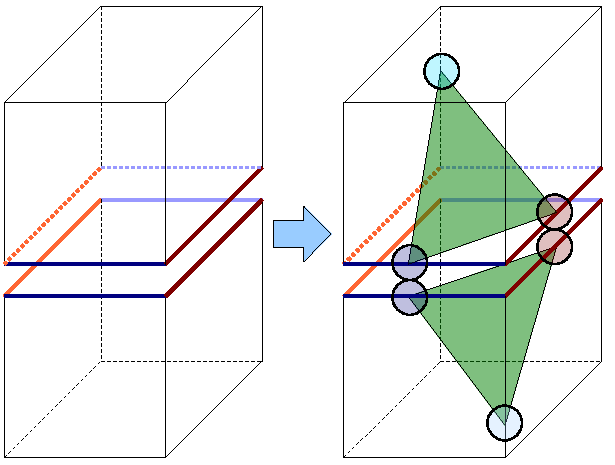
\includegraphics[height=0.3415\columnwidth]{MarchingCubesOverview.pdf}}
\subfloat[Subdivision\label{fig:teaser:subdivision}]{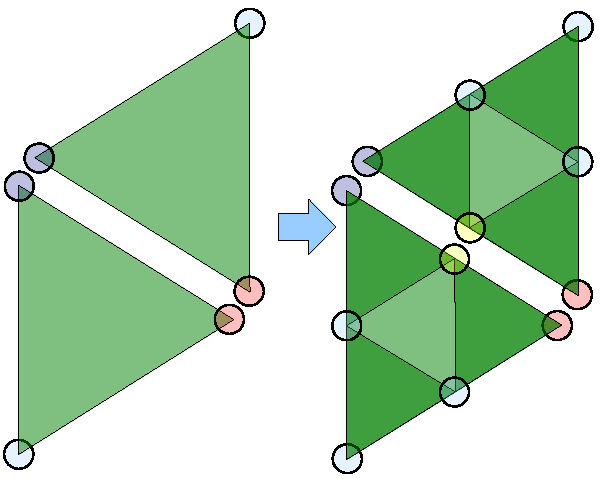
\includegraphics[height=0.3415\columnwidth]{SubdivisionExample.pdf}}
\subfloat[Face-Centered Tetrahedralization\label{fig:teaser:tetrahedral}]{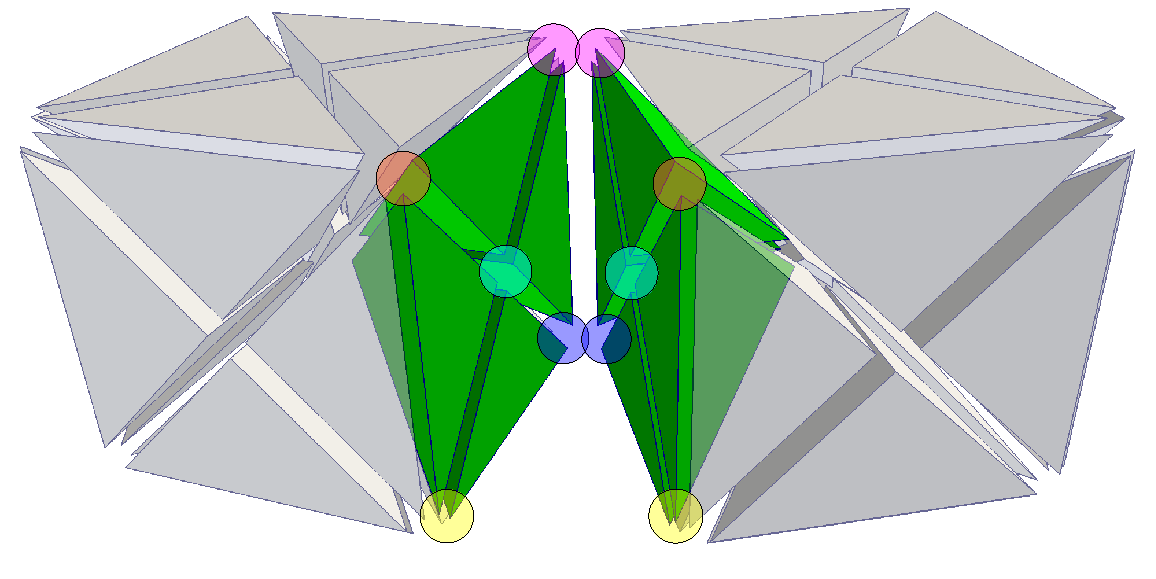
\includegraphics[height=0.3415\columnwidth]{TetrahedralExample.pdf}}
\subfloat[Dual Mesh\label{fig:teaser:dual}]{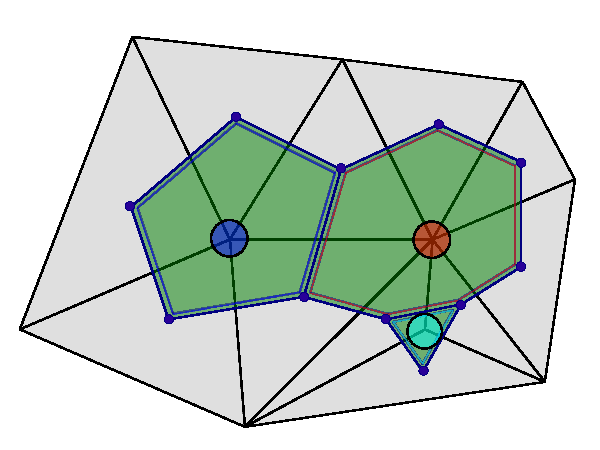
\includegraphics[height=0.3415\columnwidth]{DualMeshExample2.pdf}}
\caption{Operations that generate geometry usually rely on a known input topology for that purpose. Marching Cubes (a) generates all output vertices on the edges of a known voxel grid. By marking these output vertices with the ID of their generating edges, connectivity information can be retained. The same process can be applied to cell subdivision (b). Tetrahedralizations (c) are more complex, but still supportable by keying on the intput face as well as the input edge. Generating topology on a dual mesh (d) exchanges vertex and face connectivity information.}
\label{fig:teaser}
\end{figure*}

\noindent
\begin{minipage}{\linewidth}
To summarize, this paper makes the following contributions:
\begin{itemize}
	\item{Provide a generalized technique for generation of topological connectivity information on highly parallel systems.}
	\item{Require no modifications to the algorithms generating geometry save for the
		storage of information about the input topological features used to generate each output feature.}

	\item{Make use provenance of disconnected geometry to enhance the performance of the topology
		resolution technique.}

	\item{Demonstrate the effectiveness of our technique on the output of the Marching Cubes
		algorithm and a tetrahedralization algorithm.}
 
	\item{Show how a provenance-aware algorithmva can be used to perform
		 simple mesh coarsening in the same pass as the topology resolution.}
 
\end{itemize}
\vspace{5mm}
\end{minipage}

We developed our technique for topology resolution so that it could be implemented
into the upcoming DAX framework, which will provide data analysis capabilities similar to those
in VTK, but targeted toward massively parallel architectures, beginning with the GPU.

\section{Previous Work}
\label{sec:PreviousWork}

We use Marching Cubes as an example of parallelized geometry 
generation \cite{Lorensen1987}. There are myriad existing isosurfacing implementations on the GPU, dating from 
Rottger's implementation \cite{Rottger2000}. Dyken provides a fairly 
detailed overview of the advancements in GPU implementations of Marching Cubes and 
Marching Tetrahedra \cite{Dyken2008}.

The basic topology resolution technique described in the introduction section is
introduced by Park et al. \cite{Park}. Additionally, Kipfer mentions
implementing a topology construction technique along with their GPU
Marching Cubes algorithm \cite{Kipfer2005}. Kipfer's technique involves the use of the edges that vertices 
will be placed on as a key for determining which vertices would be duplicated. Kipfer 
thus avoids redundant computation of such vertices and avoids the need for coincident 
point resolution. To have accurate normals at the generated vertices, Kipfer's technique
requires precomputation of the gradient of the volume at the voxel vertices. Any other
interpolable attributes to be derived from the volume must also be precomputed at the
voxel vertices. Our method for determining duplicate vertices extends Kipfer's method in that
we may key off of any input feature.

Stream compaction is an important element for efficient geometry generation on the GPU.
Horn provides an early method for stream compaction on the GPU \cite{Horn2005}, which
was improved upon by Sengupta \cite{Sengupta2007}, who also provides a CUDA implementation. 
These approaches rely on the data parallelism technique and the application of prefix sums 
as described by Blelloch \cite{Blelloch1990}. Dyken further optimizes
GPU compaction techniques by making use of a data structure called a Histogram Pyramid \cite{Dyken2008}.
For our examples, we use geometry generation methods that make use of the prefix-sum
method of compaction, but other compaction techniques such as histogram pyramids could be
substituted for the prefix sum technique for increased performance in any case where our method is applied.

We use coincident point resolution (vertex welding) in Marching Cubes with the Thrust
C++ template library \cite{Bell2012}. Bell, a primary
developer of the Thrust library, also presents a vertex welding technique as an
example application of Thrust \cite{Bell2010}. Bell also notes that GPU sorting techniques can
be instrumental in the development of high-performance GPU algorithms. Hoberock uses a
lexicographic sort directly on the vertices generated by Marching Cubes, then collapses 
duplicates to get the final welded surface.

The algorithm, hereafter referred to as \proc{Vertex-Weld}, works as described in Algorithm 1.
\begin{figure}[h!]
\vspace{-0.3cm}
\begin{codebox}
  \Procname{$\proc{Vertex-Weld}(\id{vertices})$ \\
    $\id{vertices}$: Array of vertex data (i.e. coordinates).
    }
  \zi \Comment Sort $\id{vertices}$ to make identical vertices adjacent.
  \li $\id{sorted-vertices} \gets \proc{Lexicographic-Sort}(\id{vertices})$
  \zi \Comment Copy the first element from each group of duplicates.
  \li $\id{welded-vertices} \gets \proc{Unique}(\id{sorted-vertices})$
  \zi \Comment For each item in $\id{vertices}$ find the corresponding index
  \zi \Comment in $\id{welded-vertices}$.
  \li $\id{cell-connections} \gets \proc{Vectorized-Find}(\id{welded-vertices},\id{vertices})$
  \li \Return $( \id{welded-vertices}, \id{cell-connections} )$
\end{codebox}
\vspace{-0.5cm}
\caption*{Alg. 1: \proc{Vertex-Weld}, as demonstrated in the Thrust library examples, takes geometric soup as input and produces a welded topology.}
\end{figure}

\proc{Vertex-Weld} is relevant to topology reconstruction because it provides unique identities for distinct topological features, such as vertices. Prior to the operation there may exist many instances of the same topological feature. This makes it difficult to determine whether two facets connect to the same vertex, for example. After the \proc{Vertex-Weld} process is complete, it is simple to determine all facets that contain a particular vertex, which can allow computation of incidence and adjacency lists. \proc{Vertex-Weld}  can be efficiently implemented using well-studied parallel algorithms.  For example, the functions \proc{Lexicographic-Sort},
\proc{Unique}, and \proc{Vectorized-Find} are performed using the parallel
Thrust functions \texttt{sort}, \texttt{unique}, and \texttt{lower\_bound},
respectively.

Our approach has many similarities, but there are several areas of interest where \proc{Vertex-Weld} was not designed to accommodate topological reconstruction. In particular, \proc{Vertex-Weld} provides no way to make use of the provenance of the disconnected geometry. Additionally, the \proc{Vertex-Weld} algorithm as presented is unstable in the presence of floating point errors because these can cause the \proc{Lexicographic-Sort} to place 'identical' points in noncontiguous regions of memory, thus invalidating the algorithm. A more stable solution which still uses bitwise comparison can be constructed by sorting on each dimension and removing duplicates each time, but this is inefficient. Instead, we resolve both of these concerns by allowing a sort on input topological features, and a generalized comparison and merge operation with our algorithm, to be described in the next section.

Carr et al. \cite{Carr2006} describe several ways to subdivide voxel grids into tetrahedral grids. To fairly test performance of our topology generation on unstructured grids, we generate each of these subdivisions and demonstrate that the performance of our approach is similar in all cases.

Observant readers may notice a similarity between our proposed algorithms and those supported by the MapReduce framework \cite{MapReduce}. Like MapReduce, our algorithms first map keys to values then collect keys and reduce the values. Although we believe our algorithms could be implemented in a MapReduce framework (an exercise we leave to the reader), it would require additional collection operations to resolve topological connections. Other researchers 
\cite{Stuart2010}\cite{Vo2011} have implemented visualization algorithms directly in MapReduce, but they serve purposes other than those we address.

In most cases, existing GPU implementations of Marching Cubes do not determine connectivity information on output contour surfaces, but instead simply forward disconnected geometry for rendering \cite{Dyken2008} \cite{Goetz_Junklewitz_Domik_2005} \cite{Johansson_Carr_2006}. However, many serial implementations exist that determine topological connectivity information from discrete geometry. For example, VTK and ParaView make use of a point-locator method, which works by beginning with an empty search structure and progressively updating it with each point, checking for duplicates along the way. There also exist efficient implementations of similar search structures for finely threaded cases such as the GPU \cite{Zhou_Hou_Wang_Guo_2008}, but these are most applicable when the resultant structures will be used extensively as in the case of raytracing. Because operations like tetrahedralization, Marching Cubes (and other contour methods), dual mesh generation, and even simple subdivision can radically alter topology, we can not depend on the reuse of large search structures. Instead, we require a lightweight approach that can generate a new representation of topology quickly using known information from a previous representation.

Late in the paper, we describe a mesh coarsening method which improves triangle output quality over that normally provided by Marching Cubes. There are previously existing methods to obtain improved triangle quality from Marching Cubes \cite{Moore_Warren_1991}. The advantage we provide over these methods is that when topological information is also required we can also perform our coarsening technique in the same pass thus requiring no additional computational cost. 

\section{Using Topology Provenance}
\label{sec:UsingTopologyProvenance}

The essential idea behind our provenance-enabled topology construction is
to use components of the input topology as \emph{keys} in a MapReduce-like
framework as demonstrated in Figure~\ref{fig:ProvenanceFlow}.  In this
figure we have labeled the major steps of our algorithm with the analogous
component in MapReduce to facilitate the understanding for those already
familiar with this system.

\begin{figure}[htb]
  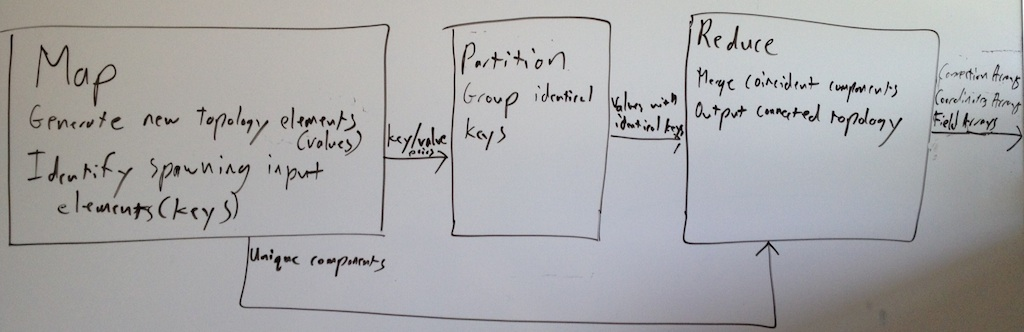
\includegraphics[width=\linewidth]{ProvenanceConstruction}
  \caption{Basic flow of an algorithm using provenance to construct
    connected topology.}
  \label{fig:ProvenanceFlow}
\end{figure}

\begin{figure*}[!tb]
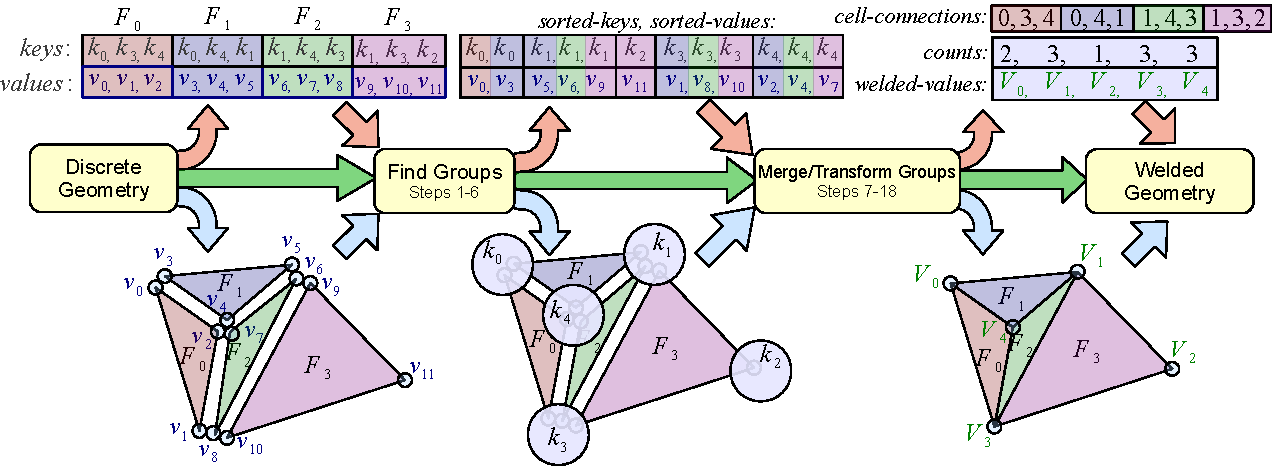
\includegraphics[width=\textwidth]{KeyWeld.pdf}
%% \caption{An example of the \proc{Key-Weld} procedure on a very small set of triangles. Data values within the algorithm at several stages are shown above the flow diagram. The represented geometry is shown below the flow diagram. Background color in the upper tables reflect the color of the associated triangle in the lower diagrams. After processing, we have a map $cell\mbox{-}connections$ that lists the new vertices for each triangle. We also have the
%% number of faces attached to each vertex in $counts$, and the welded vertices and their associated attributes in $welded\mbox{-}values.$}
\caption{An example of using topology provenance to find vertex
  connections.  A map operation, such as Marching Cubes, defines some
  collection of cells as shown at left.  A partition phase groups the keys
  and a reduce phase combines vertices and establishes a connections array
  to the new indices.  We collect the mechanisms of this process in an
  algorithm we call \proc{Key-Weld}.
  \fix{The first three yellow blocks should be changed to correspond to
    Figure~\ref{fig:ProvenanceFlow}.  Discrete Geometry, Find Groups, and
    Merge/Transform Groups should be changed to Map, Partition, and Reduce,
    respectively.}
}
\label{fig:KeyWeld}
\end{figure*}

The first step is a \emph{map} operation that generates key/value pairs
where the key is some component of the input topology and the value is a
generated component of the output topology.  In the case of Marching Cubes,
the values are the vertices generated for the new surface mesh, and each
vertex is keyed by an identifier for the edge used to interpolate the
vertex.  The map operation may also generate elements that are known to be
unique and therefore do not need keys.  For example, when subdividing
cells, some vertices come directly from the input vertices whereas others
are interpolated and must be connected.  The map operation is designed such that
key/value pairs can be generated independently, which allows us to safely
compute them concurrently on a very large pool of threads.

The second step is a \emph{partition} operation that reorganizes the
key/value pairs to group duplicate keys.  Like most MapReduce
implementations, we find a parallel sort to be an efficient way to shuffle
the data.  However, we can also take advantage of domain decompositions
when available to shorten the partitioning time.

The third step is a \emph{reduce} operation that merges groups of
coincident components identified by the partition and generates the
connected structures.  In the Marching Cubes example, this reduction means
averaging the field values on merged vertices and updating the triangle
connection indices.  Because all dependent operations are collected into
partitions, the reduce operations can also be safely computed
concurrently.

Although our system is conceptually similar to MapReduce and we believe it
possible to implement in a MapReduce framework, we choose to implement our
algorithms using the more imperative parallel operations provided by
Thrust.  This makes it easier to take advantage of known properties such as
domain decompositions or implicitly unique keys.  It also simplifies
storing topologies in efficient indexed array structures rather than
collections of key/value entities.

\section{Connecting Vertices}
\label{sec:ConnectingVertices}

Provenance can be used to identify topology elements of any type, but by
far the most common we have encountered is that of finding coincident
vertices.  Although many techniques exist to find coincident vertices, as
outlined in Section~\ref{sec:PreviousWork}, they all operate in ignorance
of any a priori knowledge.  We show that our provenance enabled technique
is both faster than existing techniques and is less susceptible to some of
the inherent limitations.

\subsection{General Merging Algorithm}
\label{sec:GeneralMergingAlgorithm}

Figure~\ref{fig:KeyWeld} provides a simple example of applying the topology
provenance technique, described in
Section~\ref{sec:UsingTopologyProvenance}, to find connections among
generated vertices.  First, a mapping operation generates the connections
for a set of cells.  Vertices are duplicated to allow independent operation
on multiple threads.  For the purposes of this paper we assume the map
operation is a previously known algorithm such as Marching Cubes with the
trivial extension that cell connection lists contain pairs of input index
(key) and output vertex (value) rather than just the output vertices.

Next, key/value pairs are partitioned by sorting the pairs based on keys.
From the sorted list of keys we can efficiently extract a list of unique
keys, which serves to identify the connected vertices to be created.  This
list of sorted unique keys can also used to look up where each original
unsorted key resides in the final list of merged vertices, which is how we
generate the $\id{cell-connections}$ array defining the cell topology.

The final step is to merge values with identical keys in the reduction
phase.  This reduction operation provides an opportunity to combine
neighborhood information such as averaging normals across surface polygons.
To facilitate averaging we also generate a $\id{counts}$ array marking
the number of cells incident to each vertex.  Although this array is not
specifically necessary to describe the final topology, it can be leveraged
to find vertex incidence lists using the algorithm proposed by \fix{cite
  whoever made the Vertex-Incidence-List algorithm}.

%% \section{Merging Algorithm}
%% Without significant modification of the algorithms generating topological features,
%% we present an approach that reconstructs the topological connections
%% between these features. By topological connections, we are referring to the information necessary to
%% determine all topological features that are adjacent to any individual feature of 
%% interest. We assume and provide a representation based on point arrays and either implicit or explicit cell connection lists. Generating incidence lists, such as the list of all cells incident to a point, is a trivial extension to our algorithm. Given a point P 
%% generated by the Marching Cubes algorithm, the topological connections
%% could be a list of all faces that contain point P as a vertex. Depending on
%% the intended use of the topology, it may be preferable to store the list of
%% points Q where there exists an edge (P,Q). Our approach can be applied
%% to generate any of these forms of connectivity information.

%% \subsection{Goals}
%% In developing our technique for reconstruction of topological connections, we have the
%% following requirements.
%% \begin{itemize}
%% 	\item{Support at least the following feature types: vertices, edges, faces and facets.}

%% 	\item{Require minimal modification to the algorithms used to generate topological features.}

%% 	\item{Work as an efficient data-parallel method}
 
%% \end{itemize}

%% \subsection{Algorithm}
%% Our technique was developed by generalizing and extending the vertex welding example from the Thrust library \cite{Bell2012}.
%% Since many vertices are redundant when all triangles in a mesh are stored discretely, it is often desirable to
%% `weld' the duplicate vertices to single instances. We base our technique on the Thrust method because it has a similar
%% structure to the approach we take for topology generation, and because it is designed to work with nVidia CUDA platforms as well as platforms supported by OpenMP. 

%% %\begin{itemize}
%% %	\item{Given an array of point coordinates $V_1$:}
%% %	\begin{enumerate}
%% %		\item{Lexicographically sort $V_1$ so that duplicate vertices are placed together in the array.}
%% %		\item{Take the first element from each group of duplicates and store it in an output array $V_2$.}
%% %		\item{Find the new index in $V_2$ for each vertex in $V_1$ and store it in an output array $Map_{1\rightarrow 2}$, which serves as a many-to-one mapping of points in $V_1$ to $V_2$.}
%% %	\end{enumerate}
%% %	\item{Return $V_2$ and $Map_{1\rightarrow 2}$ as output.}
%% %\end{itemize}

%% \proc{Vertex-Weld} is a good basis for an algorithm to generate topological connectivity because it allows for
%% grouping and processing of duplicate vertices. Since we can store which triangle generated each copy of a duplicate vertex,
%%  the above algorithm can be adapted to calculate a neighboring face list for each point. Therefore, using \proc{Vertex-Weld} as a basis, we set out to create a technique that could be used for generating topological connectivity information 
%% from multiple kinds of disconnected input geometric elements. There are several requirements for this which the \proc{Vertex-Weld} algorithm
%% does not immediately meet.

%% Unlike the creators of the \proc{Vertex-Weld} algorithm, we are not interested specifically in the elimination of duplicate elements. Instead, we want
%% to form groups of geometric elements and then merge these into an output. These elements may not be simple vertices as in the \proc{Vertex-Weld} example.
%% To use this for the generation of topological connections, we will need to associate attributes with each vertex. To this end, rather than taking as input an array of vertices,
%% we take in an array of geometric elements of some unspecified type. Often, the input will be an array of `tuples' which may consist of
%% vertices and their associated attributes such as normals or polygon IDs. Hereafter, we will refer to this input array as the `mergeable' array.

%% The \proc{Vertex-Weld} algorithm groups bitwise-equal elements together. 
%% This would be inappropriate if additional attributes were associated with
%% each sample of a given vertex. For instance, three vertices at the same location that possess different normal vectors
%% would not compare bitwise equal, but we may wish to process them as a group. To resolve this, we take as input an array of $keys$ where
%% each key corresponds to an element of the mergeable array. The key for each mergeable element will be compared against the keys for
%% other mergeable elements using a user defined comparison operator $keycomp$. $keycomp$ is required to be analagous to the less-than operator, so
%% it takes two keys as input and must return $true$ if the first element should be placed earlier in the array than the second element, and $false$
%% otherwise. If $keycomp(k_1, k_2) = false$ and $keycomp(k_2, k_1) = false$, then the elements are assumed to be part of the same group and will be merged.

%% The keys can be based off of point coordinates as is done in the \proc{Vertex-Weld} example. However, keys based on floating point numbers such as coordinates are inferior because of the large number of bits required to represent them and the high probability of small numerical errors leading to lexicographic differences. Later in this paper we present algorithms with more efficient keys.

%% Since we no longer require elements of each group to be bitwise
%% equal, we cannot simply use the first element of the group for our output vector. Instead, we will rely on two user-defined operators
%% which together will merge the grouped elements to a single output. The reason for having two operators is that some operations, such
%% as averaging, require two steps; in this case, the first operator would be a sum, and the second operator would be a divide. In our
%% implementation, we restrict the first operator, hereafter referred to as a merge, to be analogous to a sum: a binary operator that is commutative and associative. We restrict the input and output types of this operator so that it must take in two geometric elements and output a version that merges the elements' properties in some way.
%% Likewise, we restrict the second operator, hereafter referred to as a transform, to be analogous to scalar division: a binary operator taking one geometric element and the number of elements in the
%% group as input. The return type of the transformation operator is unrestricted, and the result of these transformations will be passed as the output of our algorithm. 

%% Finally, for this technique to be useful it must be possible to determine where each element of the mergeable array is mapped to in the output array. 
%% Our algorithm will therefore return an array of the new indices for each of the input elements.


%% With these modifications, we provide a generalized method named \proc{Key-Weld} that groups various 
%% types of geometric elements and then merge each group into single outputs. The workings of \proc{Key-Weld} are described in Algorithm 2.

We provide a generalized method that captures these partition and reduce
phases named \proc{Key-Weld} that groups various types of geometric
elements and then merge each group into single outputs.  The workings of
\proc{Key-Weld} are described in Algorithm 2.

%\begin{itemize}
%	\item{Given:}
%	\begin{itemize}
%		\item{An array of mergeable elements $M$}
%		\item{An array of keys $K$ of the same size as $M$}
%		\item{A key comparator $keycomp(k_1, k_2) \rightarrow bool$}
%		\item{A merging operator $merge(m_1, m_2) \rightarrow m_3$}
%		\item{A transformation operator $transform(m_1, GroupSize) \rightarrow Output$}
%	\end{itemize}
%	\begin{enumerate}
%		\item{Sort $M$ using the key array $K$ and the key comparator $keycomp$ to divide $M$ into groups.}
%		\item{Determine the new indices for each element and store them in an output array $Map_{1\rightarrow 2}$.}
%		\item{Merge the elements of each group in $M$ into single elements using the $merge$ operator and store in an array of mergeables $N$. During this process, maintain a count of the number of elements merged to form each group, storing these in an array $C$}
%		\item{Transform each element in $N$ into outputs using the $transform$ operator with the sizes from $C$ and store in an array of outputs $O$.}		
%	\end{enumerate}
%	\item{Return the output array $O$, the new index array $Map_{1\rightarrow 2}$, and the group sizes $C$ as output.}
%\end{itemize}

%To provide a more concrete example, our templated CUDA implementation of this technique using the Thrust library is available in the supplemental material.


\noindent
\begin{figure}
\vspace{-.32cm}
\begin{codebox}
  \Procname{$\proc{Key-Weld}(\id{keys},\id{values},\id{compare},\id{merge},\id{transform})$\\
    \id{keys}: An array of keys uniquely identifying elements.\\
    \id{values}: An array of mergeable elements the same size as \id{keys}.\\
    \id{compare}: A key comparator $\id{compare}(k_1,k_2) \rightarrow \const{bool}$.\\
    \id{merge}: A merging operator $\id{merge}(m_1,m_2) \rightarrow m_3$.\\
    \id{transform}: A transformation $\id{transform}(m_1,\id{size})
      \rightarrow \id{out}$.
  }
  \zi \Comment Sort \id{values} using \id{keys} to make groups.
  \li $(\id{sorted-keys},\id{sorted-values})$
  \zi \>\> $\gets \proc{Key-Sort}(\id{keys},\id{values},\id{compare})$
  \zi \Comment Determine the new indices for each element.
  \li $\id{unique-keys} \gets \proc{Unique}(\id{sorted-keys})$
  \li $\id{cell-connections} \gets \proc{Vectorized-Find}(\id{unique-keys},\id{keys})$
  \zi \Comment Get a reverse map from output array to sorted arrays.
  \li $\id{reverse-map}$
  \zi \>\> $\gets \proc{Vectorized-Find}(\id{sorted-keys},\id{unique-keys})$
  \zi \Comment Get the size of each group (one per unique key).
  \li $\id{weld-array-size} \gets \proc{Length}(\id{reverse-map})$
  \li $\id{counts} \gets \{ \}$
  \li \For $i \gets 0$ \To $\id{weld-array-size} - 2$
  \zi \Do \kw{in parallel}
  \li     $\id{counts}[i] \gets \id{reverse-map}[i+1] - \id{reverse-map}[i]$
      \End
  \li $\id{counts}[\id{weld-array-size}-1]$
  \zi \>\> $\gets \proc{Length}(\id{sorted-keys})$
  \zi \>\>\> $ - \id{reverse-map}[\id{weld-array-size}-1]$
  \zi \Comment Merge elements of each group into a single element.
  \li $\id{welded-values} \gets \{ \}$
  \li \For $\id{weld-index} \gets 0$ \To $\id{weld-array-size} - 1$
  \zi \Do \kw{in parallel}
  \li     $\id{sort-index-start} \gets \id{reverse-map}[\id{weld-index}]$
  \li     $\id{count} \gets \id{counts}[\id{weld-index}]$
  \li     $v \gets \id{sorted-values}[\id{sort-index-start}]$
  \li     \For $\id{group-index} \gets 1$ \To $\id{count} - 1$
  \zi     \Do
  \li         $\id{sort-index} \gets \id{sort-index-start}$
  \zi         \>\>\>\> $+ \id{group-index}$
  \li         $v \gets \id{merge}(\id{sorted-values}[\id{sort-index}])$
          \End
  \li     $\id{welded-values}[\id{weld-index}]$
  \zi     \>\> $\gets \id{transform}(v, count)$
      \End
  \li \Return $(\id{welded-values}, \id{cell-connections}, \id{counts})$
\end{codebox}
\vspace{-0.47cm}
\caption*{Alg. 2: The \proc{Key-Weld} procedure welds vertices and allows multiple local samples of vertex attributes to be merged to form a better sampling without non-local operation during geometry generation.}
\end{figure}

The \proc{Key-Weld} algorithm takes as its input data the result of a map
operation.  Also passed to \proc{Key-Weld} are a \emph{merge} operation, which
combines two values, and a \emph{transform} operation, which completes a
reduction from a fully merged set.  Together the merge and transform
operations allow reductions to take place iteratively, which can be
important for distributed or streaming implementations.

Our \proc{Key-Weld} algorithm is implemented wholly using the parallel
operations provided by the Thrust library.  Steps 1 through 6 use functions
that are analogous to those directly provided by thrust.
Steps 7 through 18 in \proc{Key-Weld} are described at a high level for clarity. For increased data parallelism, we actually implement this portion of the algorithm using the Thrust library's \texttt{inclusive\_scan\_by\_key} and \texttt{zip\_iterator}. An example of how this algorithm works is provided in Figure \ref{fig:KeyWeld}.

We note that the \proc{Key-Weld} algorithm combines features of both
MapReduce and \proc{Vertex-Weld}, making it a curious amalgamation between
the two.  The remainder of this section describes applications of
\proc{Key-Weld} as a typical vertex weld (albeit potentially faster than
\proc{Vertex-Weld} with a more robust coincident point comparison).
Subsequent section\fix{s?} apply the \proc{Key-Weld} algorithm in more
unique ways to identify different topological connections.

\subsection{Marching Cubes}
\label{sec:MarchingCubes}

In the case of Marching Cubes (or any variant like Marching Tetrahedra), we
know a good deal about the input topology on which the output is
generated. Specifically, the output vertices from Marching Cubes are
generated only on the edges of input voxels.

To create a provenance aware Marching Cubes, we run a typical
implementation such as \fix{cite algorithm we use}.  In addition to
recording the coordinates of each triangle vertex, we also write out an
index identifying to edge on which the vertex lies.

For a structured voxel grid, we assign each unique edge an implicit integer
index, then store the corresponding edge index for each vertex generated by
Marching Cubes.  Because the edge indices are implicit, we need neither to
create nor to store an edge list.  For unstructured grids, no such implicit
edge identifiers necessarily exist.  However, each edge is uniquely
identified by its two end vertices.  We build unique local edge indices by
concatenating these two end vertices in a canonical order (we put the
smallest vertex first).  This unstructured approach works fine for voxel
grids, but requires more bits in the indices than necessary and can thus
slow down the key sort.

The results of this keyed Marching Cubes map are completed using the
\proc{Key-Weld} process described in
Section~\ref{sec:GeneralMergingAlgorithm}, which results in a manifold
surface.  We also offer to blend other field information at the vertices.
This is particularly helpful for creating interpolated surface normals from
flat triangle normals or input gradients, which are not continuous across
cell boundaries.

\subsection{Cell Subdivision}

A simple topology-generating algorithm is that of cell subdivision, which
can be used to smooth or improve the representation of a finite element
mesh.  For example, a triangle can be divided into four sub-triangles, as
demonstrated in Figure~\ref{fig:teaser:subdivision}, or a tetrahedron can
be divided into twelve sub-tetrahedra.

As with Marching Cubes, simplex subdivision always adds vertices on edges
of the input mesh, and our subdivision algorithm incorporates the
\proc{Key-Weld} process in much the same way as Marching Cubes.  One major
difference, however, is that subdivision also reuses all the vertices from
the initial mesh whose connectivity is already known.  Thus, only the new
vertices generated on the edges should be partitioned and reduce while the
others are passed and incorporated into the output.

\subsection{Face-Centered Tetrahedralization}

There are many ways in which to divide hexahedra into tetrahedra.  One
technique known as face-centered tetrahedralization divides each hexahedron
into 24 tetrahedra by adding new vertices to each face and the center of
the hexahedron.  Although it generates many more tetrahedra than some of
its counterpart algorithms, the face-centered tetrahedralization captures
the nonlinear field well~\cite{Carr2006}.

Unlike our previous algorithms, face-centered tetrahedralization generates
new vertices on faces instead of on edges.  The only change we need for our
provenance aware approach is how we create keys for face elements.  For
voxel grids, we can implicitly index the faces is a similar way we indexed
edges.  For unstructured grids, we observe that each face can be uniquely
identified by three of its vertices.  So in this case we can represent each
face with three canonical vertices, such as the vertices with the lowest,
second lowest, and third lowest indices in that order.

\section{Mesh Coarsening}
\label{sec:coarsening}

One of the more curious attributes of provenance-enabled topology
construction is that there is flexibility in how we record the provenance,
and changing the association between input and output elements can have
interesting and useful outcomes.  In this section we describe how to alter
the provenance of the Marching Cubes algorithm to provide an effective but
free first-level coarsening of the resulting surface.

\begin{figure}[htb]
\begin{center}
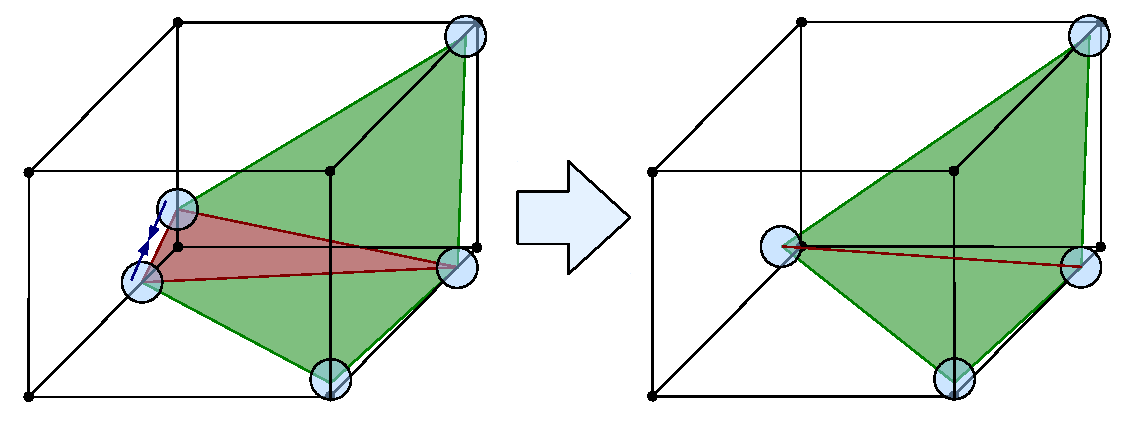
\includegraphics[width=\columnwidth]{SkinnyCollapse.pdf}
\caption{When several Marching Cubes output vertices (blue) fall close to
  the same input vertex (black), small or skinny triangles may be produced
  (red).  Merging the nearby vertices collapses the skinny triangles into
  degenerate triangles, which are then removed. }
\label{fig:SkinnyCollapse}
\end{center}
\end{figure}


%\begin{figure}[!tb]
%\begin{center}
%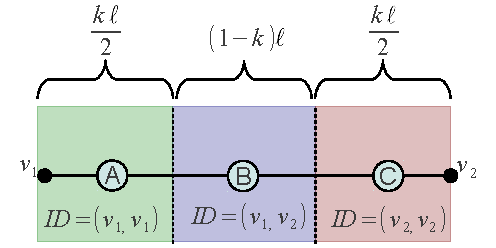
\includegraphics[height=0.5\columnwidth]{IDs.pdf}
%\caption{Our goal is to merge output vertices (light blue) that are generated too close to the vertices of the input voxel grid (black). To do so, we split each input voxel edge into three regions along edges of length $\ell$, using a control parameter $k$ to control the size. If a vertex is generated in the central region (B), we assign an output ID as normal. However, if a vertex is generated in one of the edge regions (A or C), we repeat that region's vertex ID. All output vertices generated near a particular input grid vertex are thus assigned the same ID and merged, which collapses skinny triangles to degenerate cases.}
%\label{fig:IDs}
%\end{center}
%\end{figure}

%\begin{figure}[!tb]
%\begin{center}
%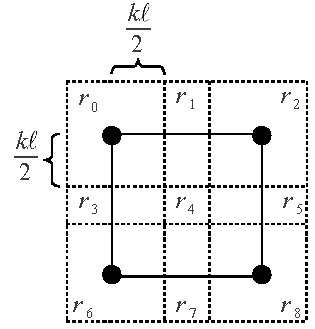
\includegraphics[height=0.5\columnwidth]{Subdivision.pdf}
%\caption{2D representation of implicit spatial subdivision into regions for the assignment of IDs to vertices generated on structured grids. Each region surrounding a voxel edge is shared by between 4 and 8 voxels. Because these regions can be determined directly from the output vertex coordinates, they need not be stored in memory. As such, no modification to the geometry generating function is required if the input voxel grid is known. Furthermore, determination of the integral region ID allows for faster sorting, as no lexicographic comparison of the vertices is required.}
%\label{fig:Subdivision}
%\end{center}
%\end{figure}


The basic idea for our coarsening is described in
Figure~\ref{fig:SkinnyCollapse}. Marching Cubes generates small or skinny
triangles when two adjacent output vertices are generated near the same
input mesh vertex.  These skinny triangles are a problematic artifact of
Marching Cubes.  They lead to poor interpolation of surface normals,
shading, and other fields as demonstrated in Figure~\ref{fig:coarsening}.
The juxtaposition of skinny and fat triangles can also cause irregularities
in their orientations, which can yield a staircase-like appearance as
evident in Figure~\ref{fig:averaging}.

\begin{figure}[htb]
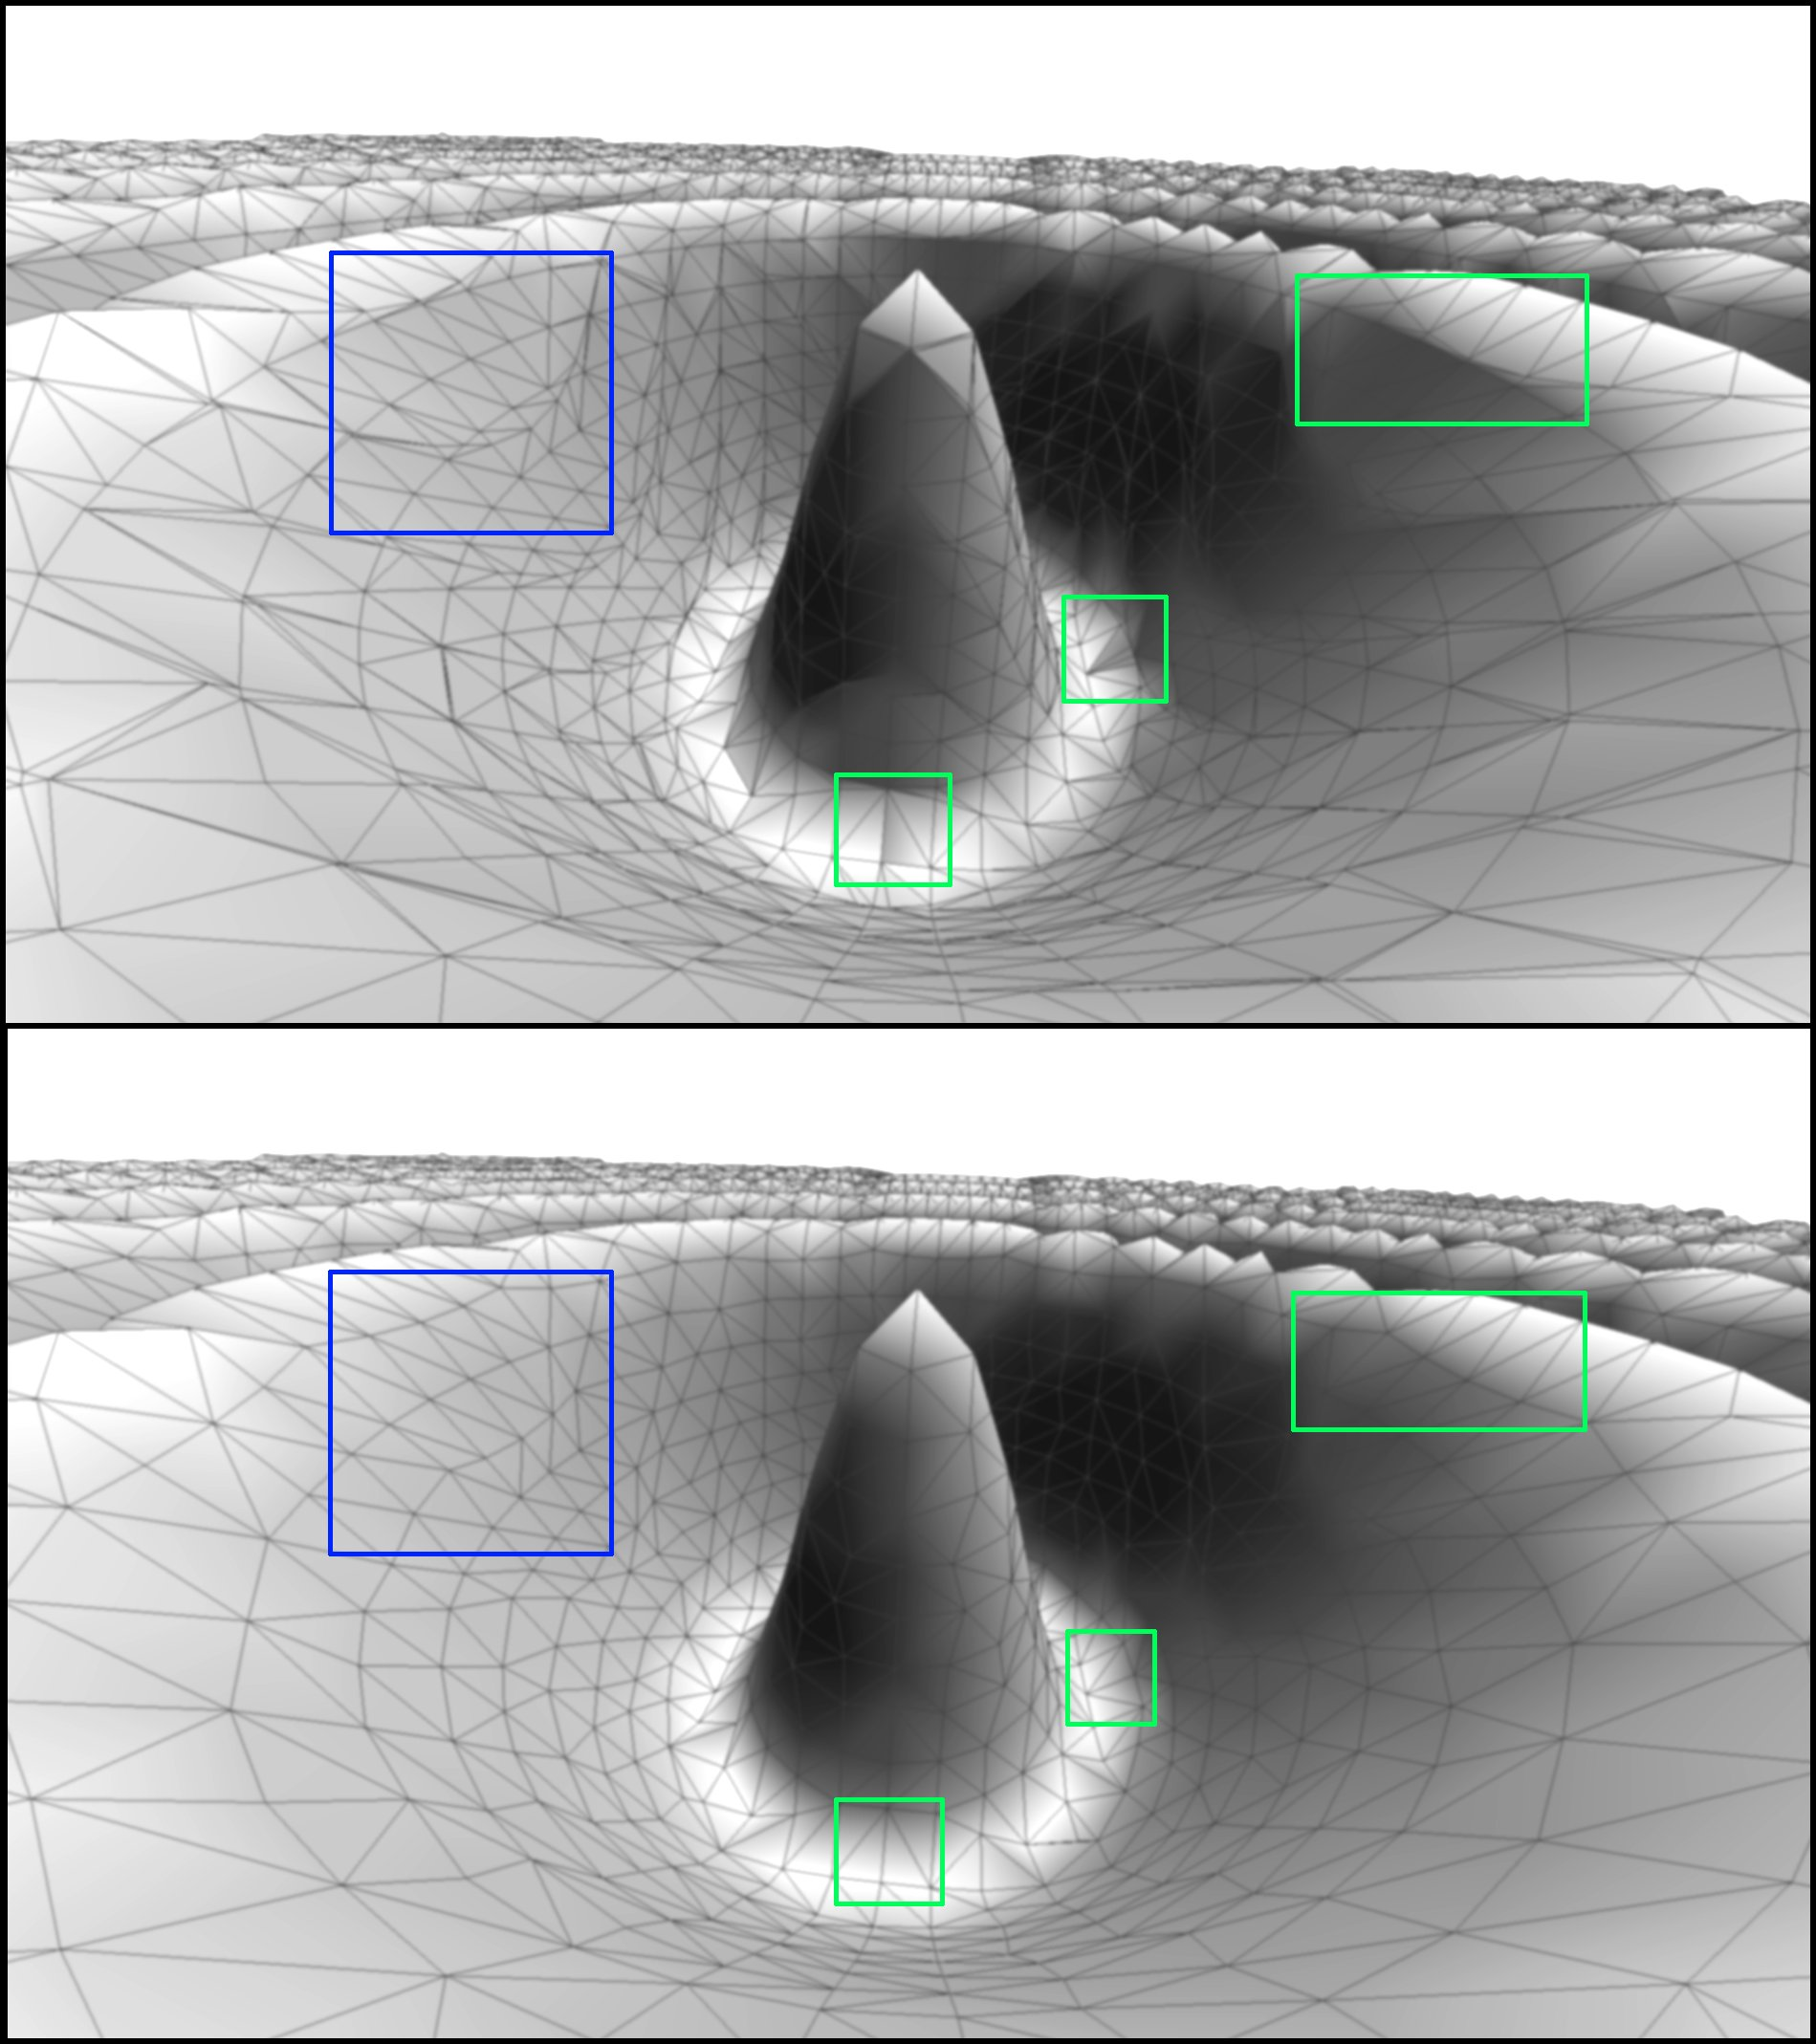
\includegraphics[width=\columnwidth]{Coarsening.jpg}
\caption{Marching Cubes output without (top) and with (bottom) coarsening.
  The blue region shows how triangle quality is improved by eliminating
  thin triangles. The green regions show improvements to surface
  interpolation made possible by removal of the thin triangles.}

\label{fig:coarsening}
\end{figure}

\begin{figure}[htb]
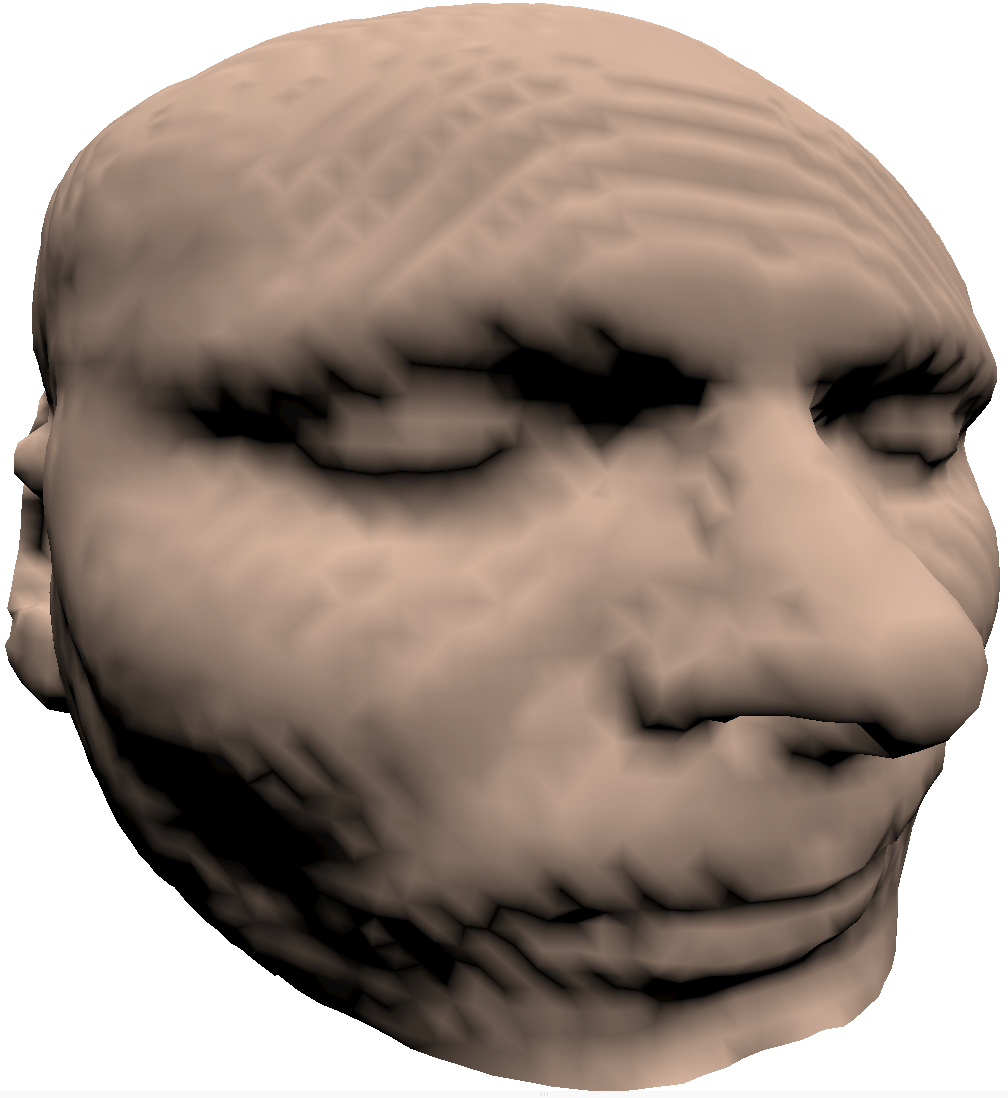
\includegraphics[width=0.32\columnwidth]{FaceNoAveraging.png}
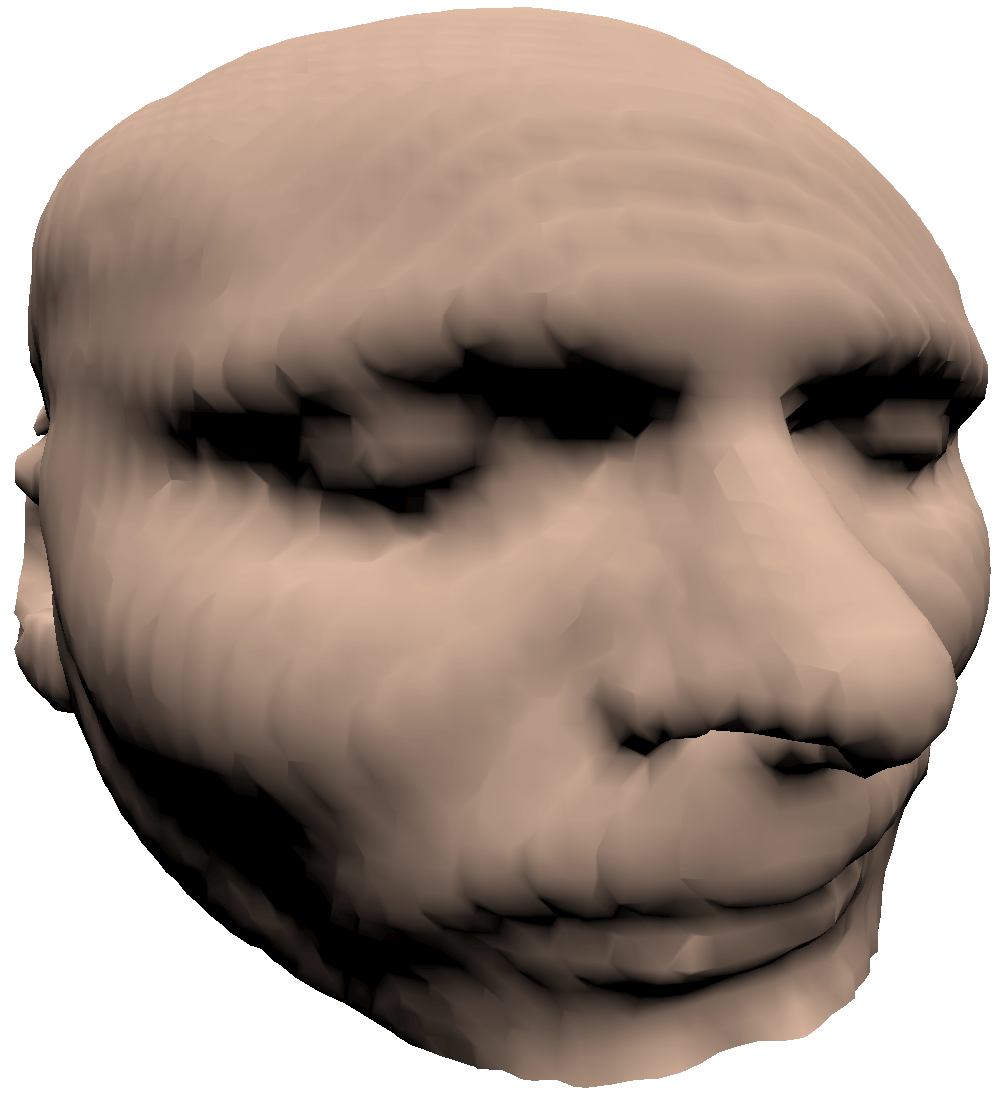
\includegraphics[width=0.32\columnwidth]{FaceAveraging.png}
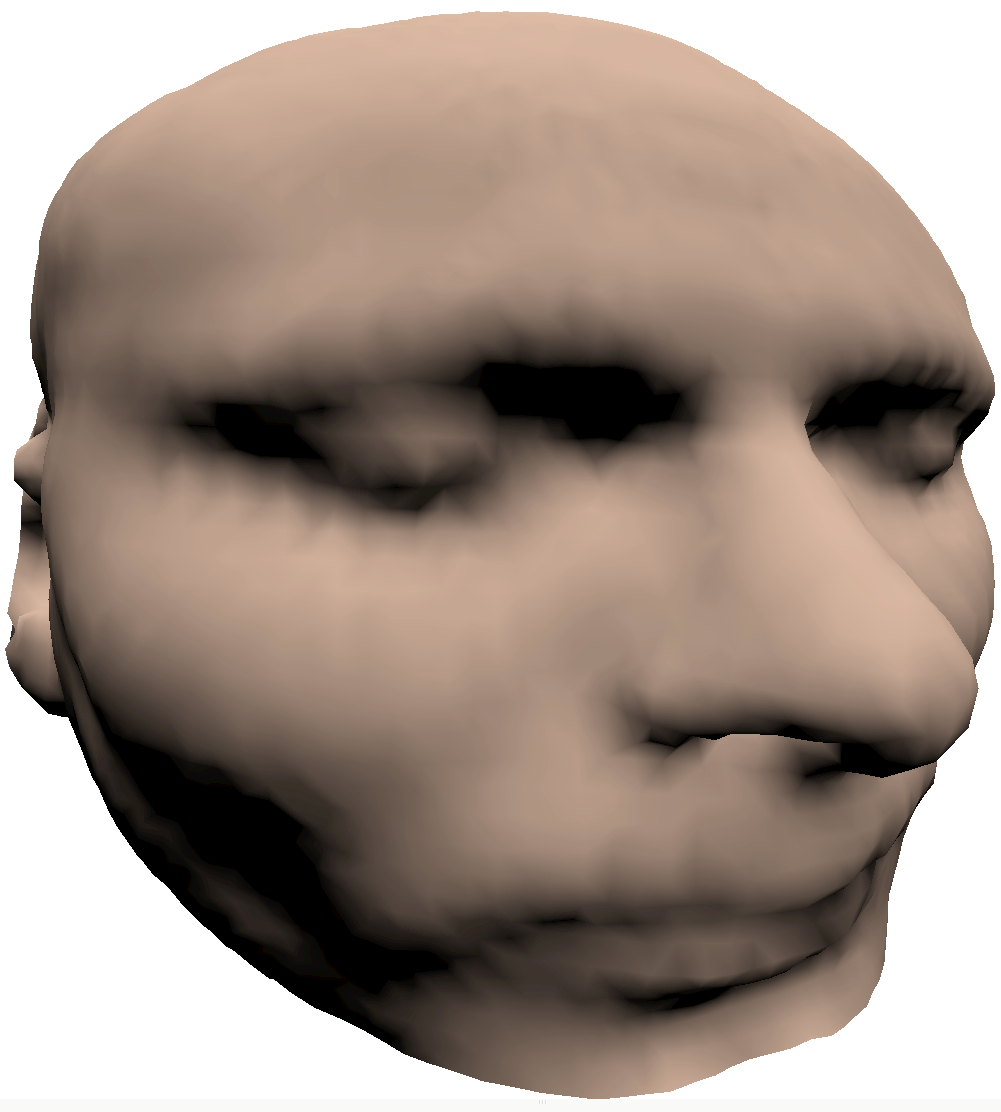
\includegraphics[width=0.32\columnwidth]{FaceCoarsening.png}
\caption{At left artifacts are visible due to sampling error caused by the
  local operation of the Marching Cubes algorithm.  At center surface
  normals are averaged on merged vertices, and smooth shading attempts to
  make the bumps less noticeable.  At right we remove these artifacts using
  our coarsening without incurring additional performance costs.  \fix{One
    thing I notice about the left image is that it does not look as if the
    shading is totally flat.  Why is that?}}
\label{fig:averaging}
\end{figure}

\begin{figure*}[htb]
\begin{center}
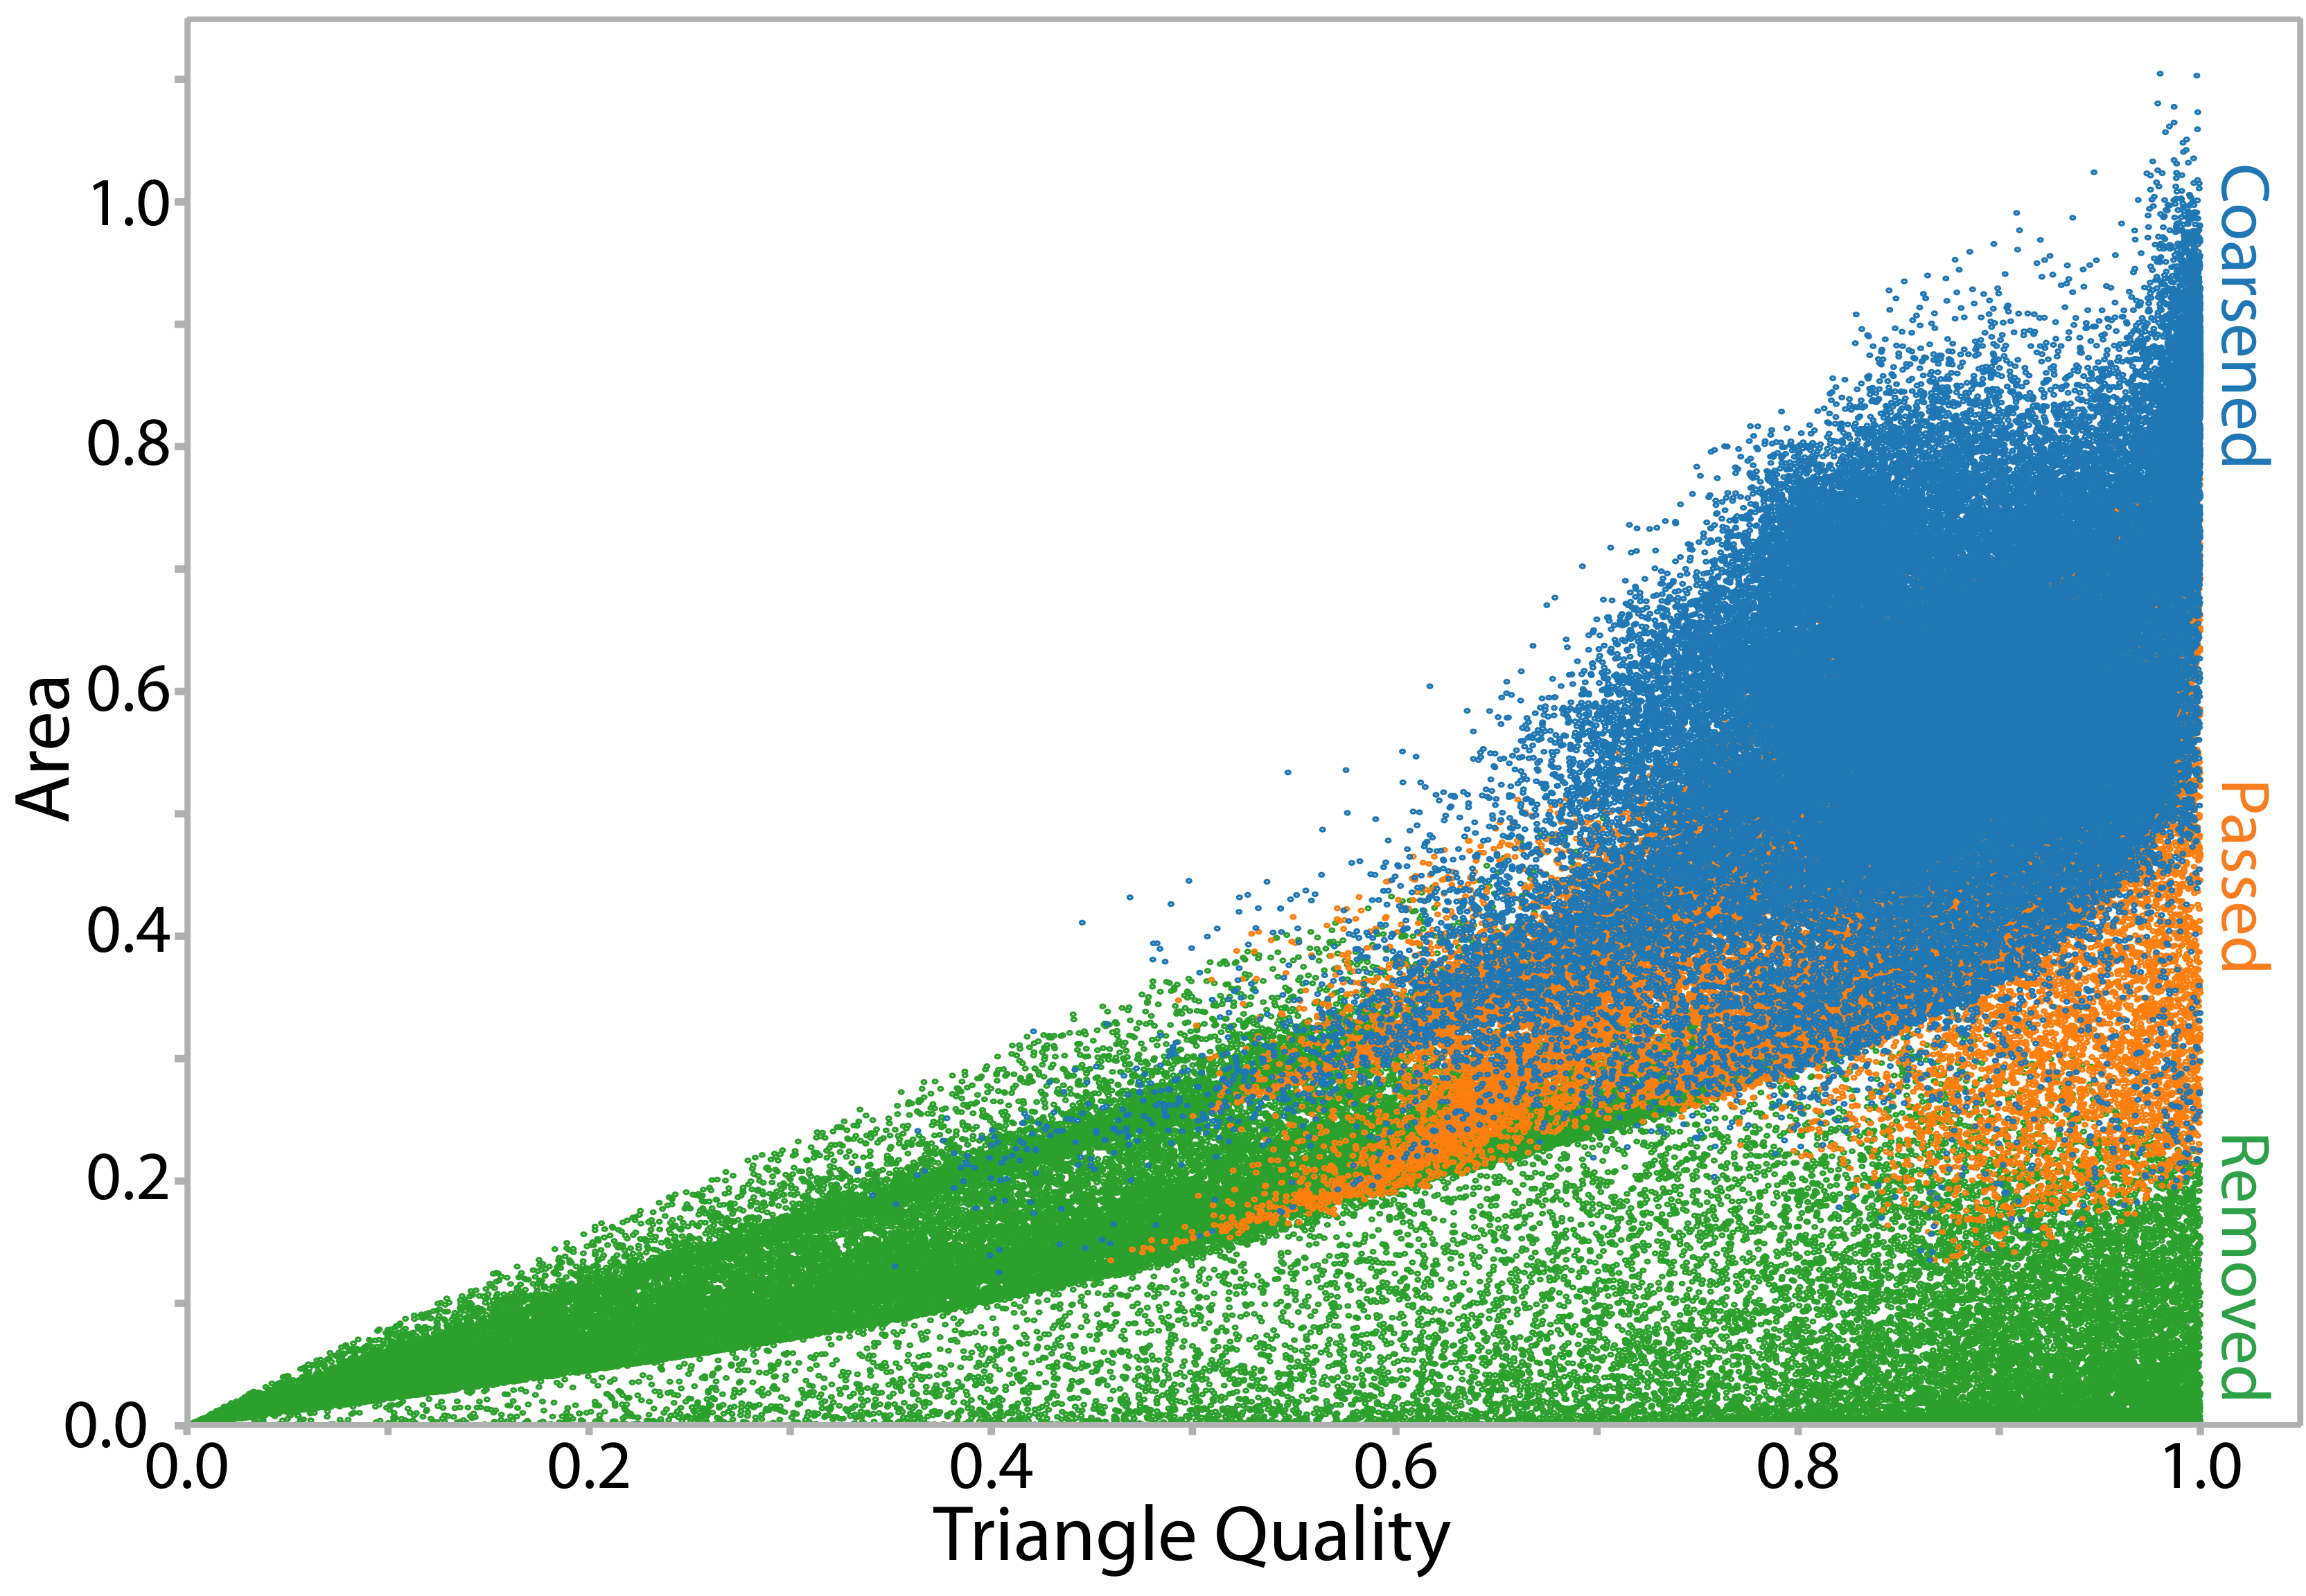
\includegraphics[height=7.05cm]{ScatterAll.png}
\hspace{0.1cm}
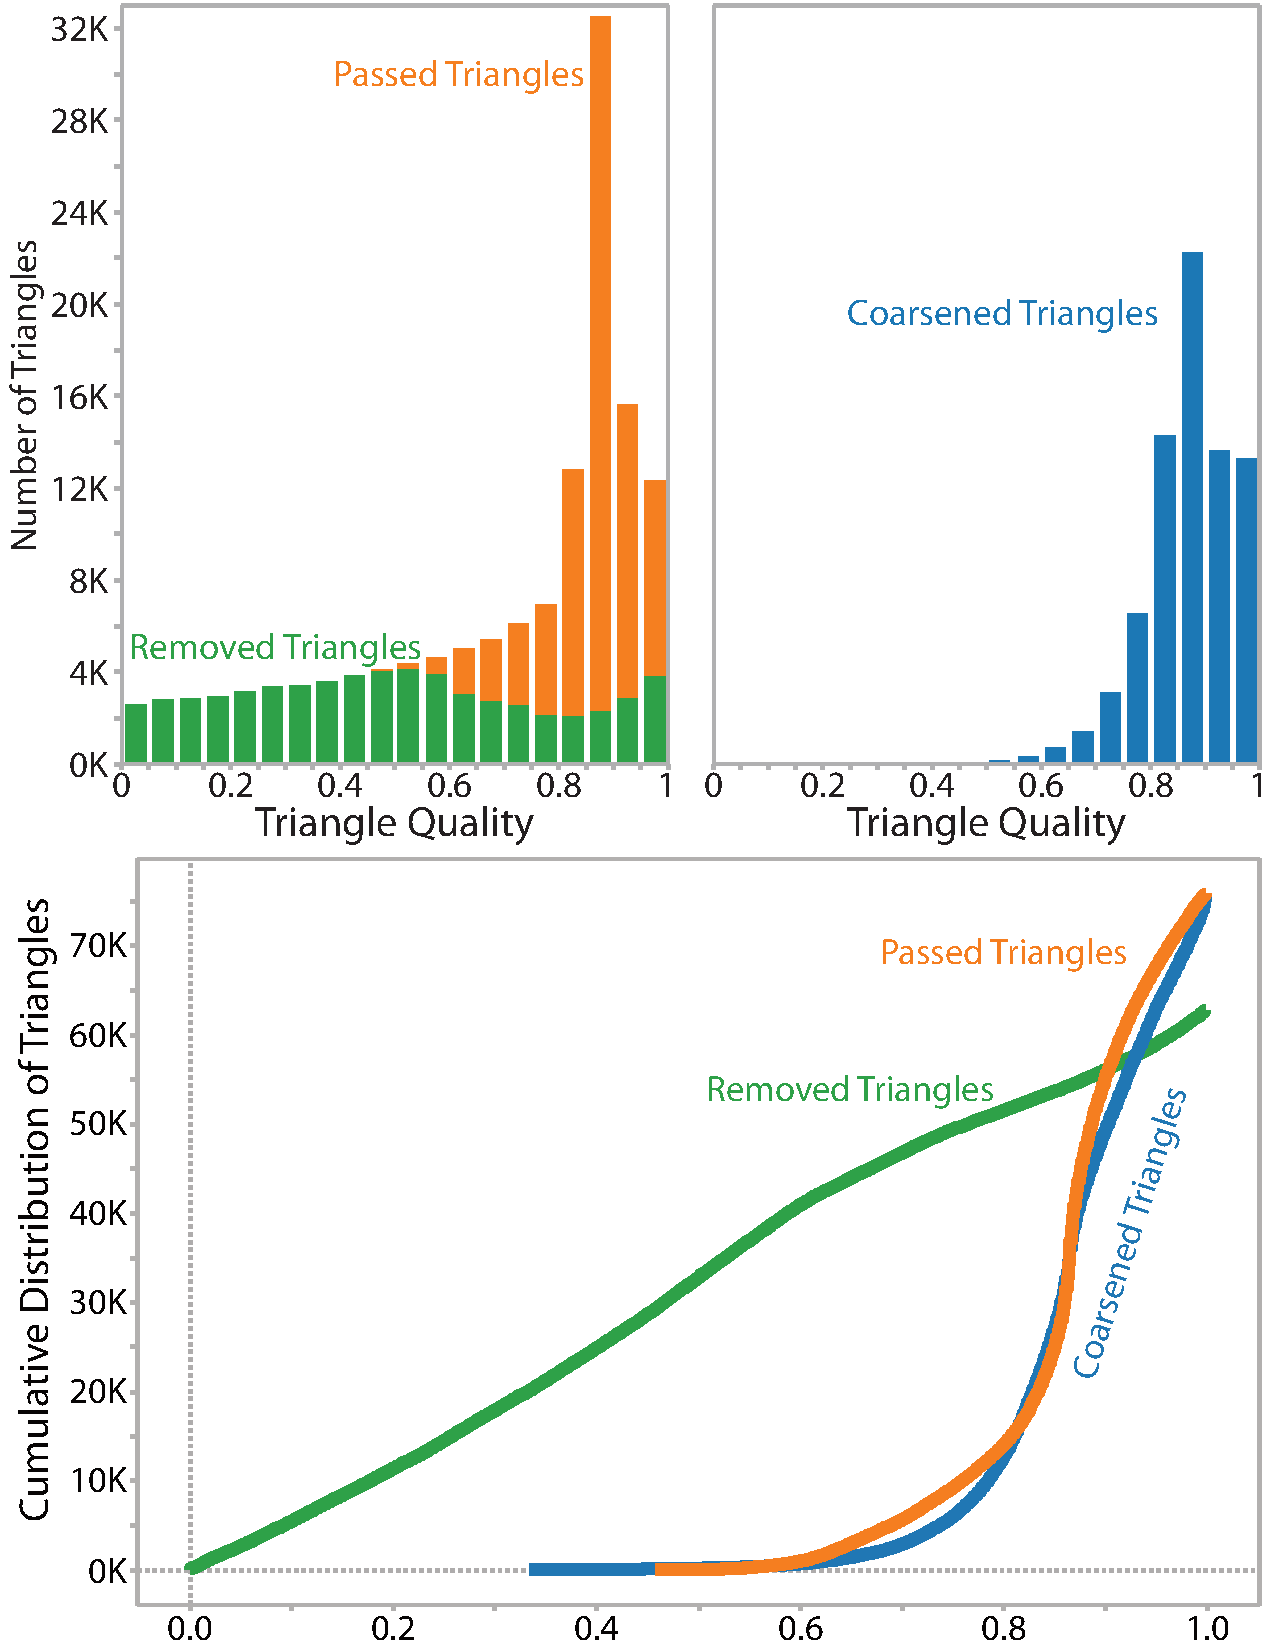
\includegraphics[height=7.05cm]{MergedFigures.pdf}
\caption{Left: Scatterplot of triangle area and triangle quality for the MRI head dataset as calculated in Eq. \ref{eq:quality}.
Top Right: Histograms of the quality of passed, removed, and coarsened triangles.
Bottom Right: Cumulative distributions of triangles before and after coarsening.}
\label{fig:coarseninggraphs}
\end{center}
\end{figure*}

The skinny triangles can be eliminated by collapsing nearby vertices.  With
provenance-enabled topology generation, this collapsing is deceptively
simple.  Rather than key each output vertex by the input edge whence it
comes, as described in Section~\ref{sec:MarchingCubes}, we key each output
vertex by the nearest input vertex connected to the input edge.  This
simple change causes the partition to group all nearby vertices and the
reduce to merge these vertices together.  When vertices are merged their
point coordinates and field values are averaged.

%% Essentially we divide the edges on which geometry is generated into three regions. We reserve a parameter $k$ to determine the size of these regions as a fraction of the edge length $\ell$. For unstructured grids, we modify the ID assignment we used previously in vertex welding. As before, we initially assign each vertex in the input topology an ID. During geometry generation, we pair these vertex IDs to form edge IDs, which are attached as attributes to the output vertex. However, when a vertex falls within $\frac{k\ell}{2}$ of an endpoint of this edge, the ID of that endpoint is repeated.

%% As with the original ID assignment for structured grids, we can use our knowledge of the input topology to assign the IDs implicitly so that there is no performance or storage cost. This is accomplished by subdividing space such that each voxel vertex falls within a unique cell and assigning an integral ID to each cell. All output vertices generated within these cells will be considered identical and merged during Vertex Welding. The value of $k$ is restricted such that $0\leq k \leq 1$, and $k$ specifies the width of the cells that will group vertices. By placing the center of these cells over the intersections of the voxel grid, the `skinny' triangles generated by Marching Cubes can be reduced or eliminated. In the structured grid case, when $k=1$ we can guarantee a minimum possible triangle quality. For cubic voxel grids, this minimum is $Q=0.275$, and the expected triangle quality is much higher, as shown in Figure~\ref{fig:coarseninggraphs}. We cannot make such a guarantee about the output of the coarsening in the unstructured grid case because the triangle quality depends on the aspect ratios of the input cells. When $k=0$ this technique is equivalent to the previous form of vertex welding. In our experience, using a value of $k=1$ provides the best results, which is equivalent to simply keying each generated vertex on the nearest input edge vertex. This allows for a faster sorting operation, so it is the approach taken for all figures and timings representing coarsening in this paper.

After the coarsening has been applied, we expect many degenerate triangles
in the output. These triangles may be quickly removed in parallel by
removing all instances of faces containing two or more identical indices.
%This invalidates the output array of group sizes $C$ from the Vertex Welding array, but a corrected group sizes $C$ can be generated by sorting the output array $cell-connections$ and performing a segmented scan to determine the number of instances of each index.

%% Many algorithms that make use of an input topology must modify that
%% topology to produce their output. To demonstrate how such an algorithm can
%% be constructed with our technique, we implement a form of simple mesh
%% coarsening.

There exist many surface coarsening algorithms.  Traditional
implementations of mesh coarsening operate without regard to the mesh's
provenance by either iteratively collapsing features \cite{Potter2011} or
collectively clustering vertices \cite{DeCoro2007}.  Our approach is
similar to those clustering vertices except that by integrating the
clustering with the partitioning we already do, we get a free first-level
coarsening without requiring a bounded-radius nearest-neighbor search or
auxiliary search structures.

%% However, by combining
%% edge collapsing with vertex welding we can provide a first-level coarsening
%% that is fast, has low error, provides well-formed cells, and adapts to the
%% structure of the original mesh.

%% Rather than computing the topological connectivity of the original
%% generated data and then coarsening it thereafter, we instead alter the
%% input key array to our Vertex Welding technique to perform a type of
%% coarsening in the process of topological connectivity generation.

Also, although our technique reduces the mesh size, philosophically
speaking we are more interested in improving the quality of the mesh than
in reducing the number of triangles, which is the primary focus of previous
work.  Specifically, it is our goal to eliminate poor quality triangles in
the mesh while performing minimal modifications to the others, without
requiring an additional processing pass. We define triangle quality $Q$ as
\begin{equation}
\label{eq:quality}
	Q = \frac{4a\sqrt{3}}{h_1^2 + h_2^2 + h_3^2},
\end{equation}
where $h_x$ are side lengths and $a$ is the triangle area. This quality
metric operates only on triangle shape, and is agnostic to triangle size.

This measure of triangle quality considers only aspect ratio, and is such
that triangles where $Q > 0.6$ are considered to be of acceptable quality,
and $Q = 1$ when the triangle is equilateral \cite{Bank2003}. This is
equivalent to the pdetriq function in MATLAB.  We use this metric to
empirically demonstrate the effectiveness of our coarsening.

Figure~\ref{fig:coarseninggraphs} demonstrates the effect of our coarsening
to the isosurface of the MRI head rendered in Figure~\ref{fig:averaging}.
In general the triangles that are removed by our coarsening (green) are
either small or poor quality as compared with other triangles in the
distribution. Triangles that are not removed by the coarsening (orange) are
altered into the output triangles (blue) when point coordinates are
averaged. Although not all passed triangles are improved by this coordinate
averaging, there is a lower bound on produced triangle quality. After
coarsening, most of the triangles are relatively large and high quality.
The cumulative triangle distributions show that our coarsening reduces the
size of the output mesh to approximately half of its original size. The
median quality of the removed triangles is approximately $Q=0.5$ whereas
the median quality of passed and output triangles is approximately
$Q=0.85$.

\begin{figure}[htb]
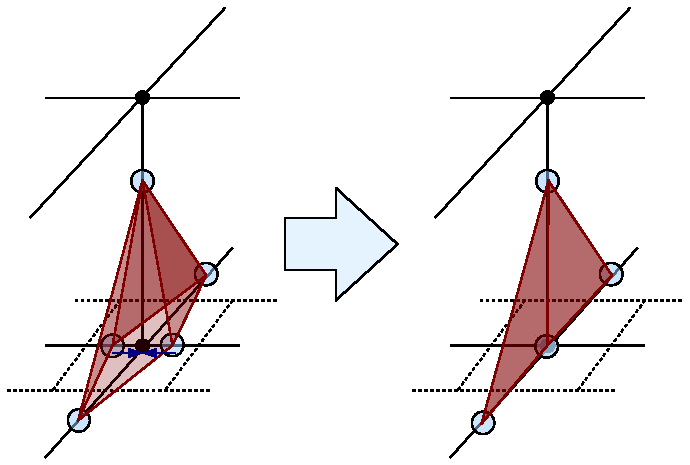
\includegraphics[width=\columnwidth]{Nonmanifold.pdf}
\caption{An example of mesh coarsening causing a non-manifold, overlapping
  surface.}
\label{fig:Nonmanifold}
\end{figure}

A problem with the coarsening technique is that in some cases, such as the
case shown in Figure \ref{fig:Nonmanifold}, non-manifold surface elements
may be generated by collapsing vertices from different parts of the
surface. In this example, two vertices from different faces are merged and
a 3D volume is collapsed into a single plane.  If such surface elements are
undesirable, they may be eliminated by calculating the maximum edge
curvature of each triangle, and removing all triangles containing an edge
curvature of $180^{\circ}$.

\section{Grouping Cell Connections}

\fix{More serious edits after this point.}

\section{Mesh Generation}
In order to test our method for generation of topological connectivities on a range of data types, we made use of several techniques to generate geometry.
To test with data calculated along a structured grid, we used the Marching Cubes algorithm to generate contour surfaces from input volume data. Next, to test
with data from unstructured grids, we tetrahedralized the volume in each of the manners as presented by Carr, et al. \cite{Carr2006}. We generated contour surfaces from these tetrahedralizations
to get similar data as from the Marching Cubes results but from an unstructured grid. Additionally, we use the tetrahedralizations directly as the input to test our technique
to find the topological connections of a 3D structure.


\subsection{Testing Environment and Datasets}

We measure performance on a test system containing an Intel Core i7 975 Processor, which has a clock speed of 3.33GHz. Our test system has 12GB of RAM, and contains 2 nVidia Tesla C2070 cards. The datasets we use for timing are shown in Table~\ref{tab:datasets}.  We do not include a tetrahedralized version of the Spherical Distance D dataset because of memory constraints. For all OpenMP tests, we set the number of threads to 8.


\begin{table}[tb!]
\begin{center}
\caption{Test Datasets}
\label{tab:datasets}
\begin{tabular}{l r r r}
\multicolumn{4}{c}{ } \\
Name & Dims &  Triangles & Tetrahedrons \\
\hline
Spherical Distance A & $64^3 $ & 35,996    & 1,250,235 \\
Spherical Distance B & $128^3$ & 149,420   & 10,241,915 \\
Spherical Distance C & $256^3$ & 607,388   & 82,906,875 \\
Spherical Distance D & $512^3$ & 2,451,212 & N/A \\
MRI Head A           & $64^3 $ & 138,510   & 1,250,235 \\
MRI Head B           & $128^3$ & 789,440   & 10,241,915 \\
MRI Head C           & $256^3$ & 4,947,294 & 82,906,875  \\
\end{tabular}
\end{center}
\end{table}


The isovalues used for contour generation are consistent for all tests within each dataset, and are chosen to show relevant features. We attach vertex normals and a scalar color value as associated attributes to each input vertex for surface contour data, but only include the color value for the tetrahedral tests due to memory constraints. In addition to the datasets listed for timings, we also use a concentric ripple dataset for some of our images for demonstration. Timings for this dataset were similar to those for the spherical dataset in all cases.

We have performed multiple tetrahedralizations as described in Carr \cite{Carr2006} to generate tetrahedral grids for input to our method, but found that our method's performance is similar in all cases. We therefore report only the timings for the minimal tetrahedralization method described in the aforementioned paper due to its smaller memory requirements. We perform Marching Cubes on each dataset to produce contour geometry. We have found that our algorithm performs similarly with output from Marching Tetrahedrons, and therefore only report the timings for Marching Cubes. All reported times in all tables are in milliseconds unless otherwise noted.  The Thrust library does not currently support spanning operations over multiple GPUs. We make use of two GPUs for our measurements by partitioning the input and performing the algorithm separately on each, then merging the results.


\subsection{Method of Topological Connectivity Construction}
Our technique is an extension of existing vertex welding methods. We will first analyze the original vertex welding approach and the manner in which we extended it for topological connectivity construction. We will then discuss methods of performance improvement of the original vertex welding method that we can achieve due to our extensions. Finally, we will discuss the usage of our extensions for the generation of topological connectivity information for various types of geometric inputs.

\subsubsection{Vertex Welding}

Because we made several modifications and extensions to the original vertex welding technique, we measure the additional performance
cost of our implementation of the technique as compared to the original. To perform a fair comparison, it is necessary to apply our technique to the same task. Vertex welding with
our \proc{Key-Weld} algorithm can be accomplished by specifying the following inputs:

\begin{itemize}
\item{The array of mergeables $values$ should be an input array of vertex coordinates.}
\item{The $keys$ array should be the same array as $values$.}
\item{The key comparator $compare$ should compare vertex coordinates lexicographically.}
\item{The $merge$ operator should simply return the first element.}
\item{The $transform$ operator should simply return the given element.}
\end{itemize}

For the purposes of vertex welding, we ignore the $counts$ output of the \proc{Key-Weld} algorithm, and treat the outputs $welded\mbox{-}values$ and $cell\mbox{-}connections$ as the original \proc{Vertex-Weld} algorithm's corresponding outputs with the same names. In this case, steps 7 through 18 can be optimized to a single call to \proc{Unique}, as in the original \proc{Vertex-Weld} algorithm. We therefore take no performance hit by generalizing \proc{Vertex-Weld} for the no-attribute case, as demonstrated in Table~\ref{tab:welding}.

Although we were able to measure the performance differences using the \proc{Key-Weld} technique, it provides no benefit over the original \proc{Vertex-Weld} in this case. Also, our generated contour surfaces contain per-vertex normals and several scalar attributes, and this approach loses all information for these associated attributes except for those related to the first encountered instance of each vertex. To resolve this, we substitute a $merge$ operator that sums these attributes, and a $transform$ operator that divides the given element by $size$ (and renormalizes in the case of the normal vector) so that our output vertices contain an averaged sample of the associated attributes from each instance of each vertex. We then measure the performance impact from this change.

\label{sec:IntegralIDs}
To improve performance over \proc{Vertex-Weld}, we make use of our ability to use input keys other than the original vertices. Initially we considered the case of the output of our structured grid
approach, Marching Cubes. In this case, we know a good deal about the input topology on which the output is generated that was not previously being used to help generate the topological connections. Specifically, the output vertices from Marching Cubes are generated only on the edges of input voxels. Each of these edges is shared by at most four voxels (ignoring degenerate vertex intersections), so there can be at most four instances of any one vertex.
We assign each unique edge in the voxel grid an implicit integer ID, then store the corresponding edge ID for each vertex generated by Marching Cubes. There is no additional storage requirement because the ID can be implicitly determined from vertex position, but even when doing so this modification causes no measurable change in the performance of geometry generation. It does, however, significantly improve performance during vertex welding. Because it is known that these IDs are identical if and only if the vertices are identical, we hypothesize that by using these integer IDs as the $keys$ in the \proc{Key-Weld} algorithm we noticeably improve the performance of the technique due to the simpler $compare$ operation used during \proc{Key-Sort}, \proc{Unique}, and \proc{Vectorized-Find}. 

We next consider the case of unstructured grid inputs. In this case edges cannot in general be implicitly assigned IDs, so they must be built from vertex IDs, which are implicit. We pair vertex IDs (least to greatest) to form a unique integral ID for each edge of the unstructured grid and store this as an attribute of each output vertex. 

Using the integer ID approach described above carries an additional advantage. From our Marching Cubes and Marching Tetrahedra implementations, we find that the \proc{Vertex-Weld} approach often fails to weld meshes as expected. We trace this failure to the fact that some vertices that should be identical actually differ slightly due to floating point error, and thus are not bitwise equal as required by the \proc{Vertex-Weld} approach. Such errors are exceptionally easy to encounter: since floating-point operations are not associative, these errors can be generated simply by failing to ensure that we always use the same vertex order when generating interpolants. By assigning integral IDs to the output vertices, \proc{Key-Weld} becomes agnostic to such floating-point error in the input vertices, and thus does not require careful prevention of these errors in the geometry-generating implementation.


\subsubsection{Vertex Welding Results}
We measure performance of the \proc{Vertex-Weld} example on each set of generated geometry. Additionally, we measure \proc{Key-Weld} with and without merging of vertex properties, and with and without the integral IDs as $keys$ to each vertex. Even when explicitly storing IDs in memory, the difference in recorded times for geometry generation are negligible for both structured and unstructured grids as opposed to the timings when these IDs are not generated. Because of this, and because geometry generation is independent of our technique, we do not report timings for geometry generation here. We report the CUDA and OpenMP timings for each approach for vertex welding on the 512x512x512 spherical dataset in Table~\ref{tab:welding}.

\begin{table}[tb!]
\begin{center}
\caption{Performance comparison for different approaches to Vertex Welding}
\label{tab:welding}
\begin{tabular}{l r r r}
%\multicolumn{4}{c}{ } \\
Test & CUDA & OpenMP \\
\hline
\proc{Vertex-Weld} (no attribute merging) & 281 & 1557 \\
\proc{Key-Weld} (no attribute merging) & 281 &  1557 \\
\proc{Key-Weld} (with attribute merging) & 527 & 2862\\
\proc{Key-Weld} (integral IDs, no merging) & 204 & 1620 \\
\proc{Key-Weld} (integral IDs, merging) & 350 & 2516 \\
\end{tabular}
\end{center}
\end{table}

Because the timings are best for merging when using integral edge IDs as keys for vertex welding when merging is necessary, all further timings in this paper use that approach for the vertex welding component. \proc{Key-Weld} reduces to \proc{Vertex-Weld} when no attribute merging is performed, so the timings are identical. Also note that using integral IDs for the non-merging case with \proc{Key-Weld} yields better performance in CUDA than \proc{Vertex-Weld}, due to the less complex comparison operator within the sort. 

The OpenMP non-merging case does not appear to benefit from the use of integral IDs. Timings for the \proc{Key-Weld} technique for Marching Cubes contours of all input datasets are shown in Table~\ref{tab:vertexwelding}, and timings when using tetrahedralizations of the input dataset are shown in Table~\ref{tab:vertexweldingtetrahedra}

\begin{table}[tb!]
\begin{center}
\caption{\proc{Key-Weld} timings for contours on structured grids.}
\label{tab:vertexwelding}
\begin{tabular}{l|r r r r|r r r}
\multicolumn{8}{c}{ } \\
 & \multicolumn{4}{|c|}{Spherical Distance} & \multicolumn{3}{|c}{MRI Head}\\
Arch. & $64^3$ & $128^3$ & $256^3$ & $512^3$ & $64^3$ & $128^3$ & $256^3$\\
\hline
CUDA & 7 & 23 & 254 & 349 & 22 & 116 & 755 \\
OpenMP & 30 & 125 & 550 & 2516 & 115 & 695 & 3377 \\
\end{tabular}
\end{center}
\end{table}

\begin{table}[tb!]
\begin{center}
\caption{\proc{Key-Weld} timings for tetrahedra.}
\label{tab:vertexweldingtetrahedra}
\begin{tabular}{l|r r r|r r r}
\multicolumn{7}{c}{ } \\
 & \multicolumn{3}{|c|}{Spherical Distance} & \multicolumn{3}{|c}{MRI Head}\\
Arch. & $64^3$ & $128^3$ & $256^3$ & $64^3$ & $128^3$ & $256^3$\\
\hline
CUDA & 127 & 1137 & 9301 & 128 & 1136 & 9322 \\
OpenMP & 1228 & 11677 & $>5$min & 1231 & 11655 & $>5$min \\
\end{tabular}
\end{center}
\end{table}

The performance of the technique appears to be bound by the number of vertices passed as input. In all cases, performance scales approximately with the number of input vertices. 

The tetrahedral case achieves approximately twice the performance per vertex of the contour case because of the absence of the normal vector as an attribute. The OpenMP version scales similarly to the CUDA version until system memory is exceeded in the largest tetrahedral dataset, at which point disk thrashing occurs during the sorts.

\subsubsection{Incidence and adjacency list construction}
\label{sec:topology}
When only considering vertex welding, we make no use of the output $counts$ of \proc{Key-Weld}, which contains the sizes of the merged groups. This output is more useful when we wish to determine the topological connections between the merged elements in $welded\mbox{-}values$. 

\noindent
\begin{minipage}{\linewidth}
We demonstrate the use of our \proc{Key-Weld} technique as a basis for determination of the following kinds of topological connectivity information:

\begin{itemize}
\item{Lists of adjacent vertices and incident edges, faces and tetrahedra for each input vertex}
\item{Lists of faces incident to each edge or adjacent to each face, even those connected only by a single vertex}
\item{Lists of faces adjacent to each face, sharing exactly one edge}
\item{Lists of tetrahedra adjacent to each tetrahedron, including those connected only by an edge or point}
\item{Lists of tetrahedra adjacent to each tetrahedron, sharing exactly one face}
\end{itemize}
\vspace{0.2cm}
\end{minipage}

We begin with a procedure \proc{Vertex-Incidence-Lists} for the generation of incident faces for each input vertex on a generated surface. 

%Example input is provided in Figure~\ref{fig:IncidenceList}.
%\begin{figure*}[!tb]
%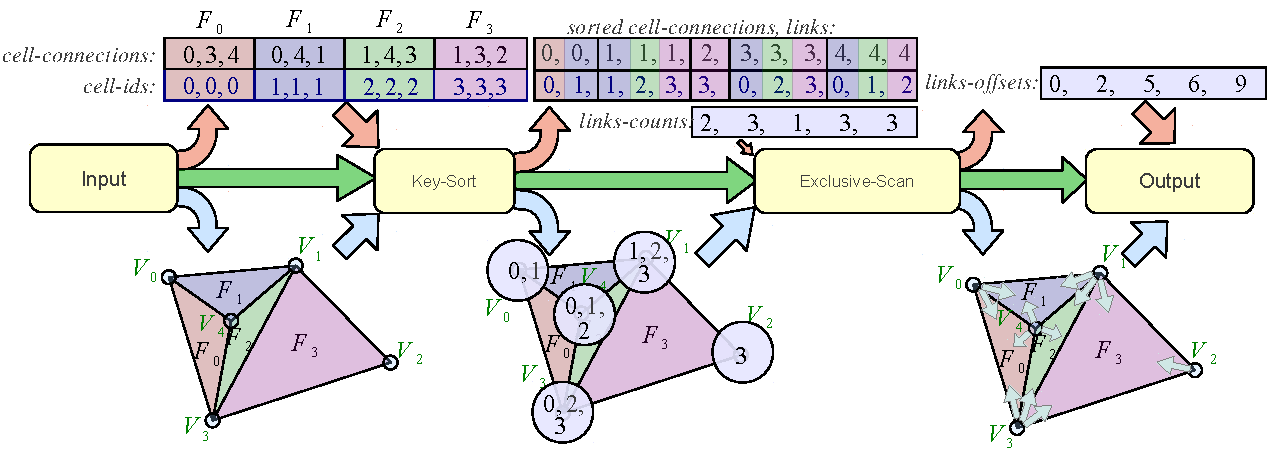
\includegraphics[width=\textwidth]{IncidenceList.pdf}
%\caption{An example of the \proc{Vertex-Incidence-Lists} procedure on a very small set of triangles. Data values within the algorithm at several stages are shown above the flow diagram. The numbers shown in the green bubbles represent \emph{values (cell-ids)}, not \emph{keys} as in the \proc{Key-Weld} algorithm in Figure~\ref{fig:KeyWeld}. Upon output, $links\mbox{-}offsets$ contains offsets to the beginning of each vertex's face list in $links$.}
%\label{fig:IncidenceList}
%\end{figure*}

\noindent
\begin{figure}[hb]
\vspace{-0.4cm}
\begin{codebox}
  \Procname{$\proc{Vertex-Incidence-Lists}(\id{cell-ids},\id{cell-connections},\id{counts})$\\
    \id{cell-ids}: An array of cell identifiers for each cell vertex.\\
    \makebox[.2in]{}Usually sequential repeated indices (e.g. $\{0,0,0,1,1,1,...\}$)\\
    \id{cell-connections}: Result from \proc{Key-Weld} representing cell connectivity.\\
    \id{counts}: Result from \proc{Key-Weld}, number of cells per vertex.\\
  }
  \zi \Comment Use a key-sort with cell connections as the keys to
  \zi \Comment group cell identifiers by vertices.
  \li $(-, \id{links}) \gets \proc{Key-Sort}(\id{cell-connections},\id{cell-ids})$
  \zi \Comment The size of each incidence list is the same as \id{count}.
  \li $\id{links-counts} \gets \id{counts}$
  \zi \Comment Use an exclusive scan to find the offset to the incidence
  \zi \Comment list for each vertex.
  \li $\id{links-offsets} \gets \proc{Exclusive-Scan}(\id{links-counts})$
  \li \Return $(\id{links},\id{links-counts},\id{links-offsets})$
\end{codebox}
\vspace{-0.4cm}
\caption*{Alg. 3: \proc{Vertex-Incidence-Lists} takes the output of the \proc{Key-Weld} algorithm and quickly generates an incidence list, represented as an array of \emph{cell-ids} and an array of pointers into \emph{cell-ids} called \emph{links-offsets} that represents the start of each cell's incidence list.}
\end{figure}

%\begin{itemize}
%\item{Generate an array $F$ containing the ID of the face represented by each instance of each vertex. For a triangular mesh, such an array would normally have the form  $\lbrace0,0,0,1,1,1,2,2,2...\rbrace$, and thus can be generated implicitly. More complex meshes may require the IDs to be generated during geometry generation, which requires extra storage but is computationally trivial.}
%\item{Perform Vertex Welding via our previously described method, using $M$ to merge any associated attributes and with $K$ being the integral IDs assigned per-vertex described in \ref{sec:IntegralIDs}. $F$ is not passed into this method.}
%\item{Use the output array $Map_{1\rightarrow 2}$ from the group merging operation in the previous step as a key to sort both $F$ and $Map_{1\rightarrow 2}$ by the elements in $Map_{1\rightarrow 2}$. }
%\item{Perform an exclusive scan on the output array $C$ from the group merging operation, storing the result in $I$.}
%\item{The output incident face list is represented by our outputs $F$, $I$, and $C$. Elements in $F$ represent faces incident to specific vertices. Elements in $I$ represent the indices in $F$ where face lists for individual vertices begin. The elements in $C$ represent the sizes of the face lists in $F$ pointed to by $I$.}
%\end{itemize}

Though our example input $cell\mbox{-}ids$ is for triangular faces, this process can be trivially extended by modifying the array $cell\mbox{-}ids$ to represent other polygonal faces, tetrahedra or any other cell type. To determine edges surrounding a point, the process could be similarly modified to have each item in $cell\mbox{-}ids$ label the represented edge. Note that when surrounding tetrahedra are generated for each vertex, surrounding faces are also generated as a subset. Similarly, when surrounding faces are generated surrounding edges are generated as a subset, which can be used to quickly determine the nearest neighboring vertices for each input vertices where an edge exists between the two.

Marching Cubes and Marching Tetrahedra both have the property that all generated surface geometry forms a manifold, with the exception of degenerate and boundary cases. Because of this, we can determine more information about the neighboring geometric features. To determine all faces touched by an edge, simply combine the incident face lists of the two endpoints. If only the two faces separated by the edge are desired, these can be detected because they will occur twice in the list. All other faces will occur only once. 

Determination of adjacent face lists for each triangular face works similarly to edges. Combine the incident face lists of all three endpoints. The face that appears three times in the combined list is the current face. Faces that occur twice are separated from this face by an edge, and those that appear only once are separated by a point.
Likewise for tetrahedra: The tetrahedron that appears four times in the resultant list is the current tetrahedron, those that appear three times are adjacent to it through a face, those that appear twice are adjacent to it through an edge, and those that appear once are adjacent to it through a point. Similar behavior occurs for other types of polyhedra and polygons.

Although the optimizations used to perform \proc{Key-Weld} change depending on whether the input is a structured or unstructured grid, the output is processed into topological connectivity information in the same manner for either case.

\subsubsection{Incidence and adjacency list construction results}
The time necessary to generate incidence lists for contours of structured and unstructured grids is shown in Table~\ref{tab:toptimings}. The time necessary to generate incidence lists for tetrahedral volumes is shown in Table~\ref{tab:toptimingstetra}.

\begin{table}[tb!]
\begin{center}
\caption{Timings for \proc{Vertex-Incidence-List} for contours on structured (SG) and unstructured (UG) grids.}
\label{tab:toptimings}
\begin{tabular}{l|r r r r|r r r}
\multicolumn{8}{c}{ } \\
 & \multicolumn{4}{|c|}{Spherical Distance} & \multicolumn{3}{|c}{MRI Head}\\
Arch. & $64^3$ & $128^3$ & $256^3$ & $512^3$ & $64^3$ & $128^3$ & $256^3$\\
\hline
CUDA & 1 & 2 & 6 & 25 & 2 & 7 & 47 \\
OpenMP & 6 & 32 & 125 & 563 & 33 & 191 & 1213 \\
\end{tabular}
\end{center}
\end{table}

\begin{table}[tb!]
\begin{center}
\caption{Timings for \proc{Vertex-Incidence-List} on tetrahedra.}
\label{tab:toptimingstetra}
\begin{tabular}{l|r r r|r r r}
\multicolumn{7}{c}{ } \\
 & \multicolumn{3}{|c|}{Spherical Distance} & \multicolumn{3}{|c}{MRI Head}\\
Arch. & $64^3$ & $128^3$ & $256^3$ & $64^3$ & $128^3$ & $256^3$\\
\hline
CUDA & 15 & 139 & 1141 & 16 & 142 & 1128 \\
OpenMP & 378 & 3610 & $>5$min & 371 & 3621 & $>5$min \\
\end{tabular}
\end{center}
\end{table}

Performance for generation of incidence lists scales approximately linearly with the number of input vertices for CUDA. OpenMP scales similarly to CUDA until system memory is exceeded in the largest tetrahedral dataset.

\section{Applications}
To test that the generated incidence and adjacency lists are useful on parallel systems once generated, we implement several calculations that make use this topological connectivity information. Specifically, we have implemented the following:

\begin{itemize}
\item{Local averaging of vertex attributes}
\item{A form of mesh coarsening, implemented as an extension to \proc{Key-Weld} without incurring additional performance cost}
\item{Generation of a dual mesh}
\end{itemize}

The local averaging technique is an example that does not alter the topological connectivity information, and thus does not require an additional application of our technique after its completion. Mesh coarsening is an example that alters the input topology, and thus requires a regeneration of the topological connectivity information after its completion. Also, we use mesh coarsening to demonstrate that certain types of mesh processing can occur during the vertex welding phase of topological connectivity construction. Generation of a dual mesh is an example that generates a new topology.

\subsection{Local Averaging}

We perform a simple averaging of properties of the nearest neighboring vertices surrounding each processed vertex. This is accomplished by first obtaining the list of indices to neighboring points as described in \ref{sec:topology}. Duplicates in this list are removed, then the attributes of each are stored. We perform a segmented scan \cite{Blelloch1991} to sum the properties of the neighboring vertices using a merge operator that is appropriate for the property type, then divide the summed properties by the number of neighbors for the group. Some vertex properties, such as normals, need an alternative operator to replace the division operation. Since we implemented our approach as a C++ template, this operator can be specified as a template parameter.

\subsection{Local Averaging Results}

Table~\ref{tab:timingsaverage} shows the timings for calculating the local averages of vector properties on the generated surfaces. Figure \ref{fig:averaging} shows a before and after comparison of averaging used for vector averaging.

\begin{table}[tb!]
\begin{center}
\caption{Timings for local averaging of scalar (S) and vector (V) properties on contour surfaces}
\label{tab:timingsaverage}
\begin{tabular}{l|r r r r|r r r}
\multicolumn{8}{c}{ } \\
& \multicolumn{4}{|c|}{Spherical Distance} & \multicolumn{3}{|c}{MRI Head}\\
Type & $64^3$ & $128^3$ & $256^3$ & $512^3$ & $64^3$ & $128^3$ & $256^3$\\
\hline
(S) CUDA & 18 & 47 & 158 & 650 & 44 & 51 & 203 \\
(V) CUDA & 18 & 48 & 158 & 649 & 45 & 51 & 203 \\
(S) OMP & 39 & 180 & 905 & 4035 & 184 & 1391 & 8611 \\
(V) OMP & 39 & 181 & 914 & 4039 & 191 & 1390 & 8625 \\
\end{tabular}
\end{center}
\end{table}

Performance for averaging scales approximately linearly with the number of input vertices in all cases. We have profiled the performance of the algorithm and found that approximately 96\% of the time taken is spent removing duplicate vertices from the incidence lists. Generation of the incidence list is the next largest fraction of the processing time, at 3\%. The time taken to perform the sum and divide operations is negligible.


\subsection{Mesh coarsening}

\subsection{Mesh Coarsening Results}
Figure \ref{fig:coarsening} shows a before and after comparison of our coarsening technique with $k=1$. 
Figure \ref{fig:coarseninggraphs} shows the change in triangle quality before and after coarsening.
Table~\ref{tab:timingscoarsening} shows the timings for coarsening the mesh as part of the vertex welding algorithm. Compare with Table~\ref{tab:vertexwelding} to observe that simultaneously performing the coarsening operation does not significantly affect the timing of the topology generation. In addition, sampling of vertex attributes is markedly improved in the coarsened graph. Although our Marching Cubes algorithm strictly determines surface normals by the information given in a single voxel, we find that our approach yields similar quality surface normals to those generated by the VTK Marching Cubes algorithm, which visits neighboring voxels to determine accurate normals. This is advantageous because it allows for completely local operation during geometry generation without loss of computed attribute quality, which provides better performance on the GPU.

\begin{table}[htb!]
\begin{center}
\caption{Timings for mesh coarsening of surface contours during vertex welding}
\label{tab:timingscoarsening}
\begin{tabular}{l|r r r r|r r r}
\multicolumn{8}{c}{ } \\
 & \multicolumn{4}{|c|}{Spherical Distance} & \multicolumn{3}{|c}{MRI Head}\\
Arch. & $64^3$ & $128^3$ & $256^3$ & $512^3$ & $64^3$ & $128^3$ & $256^3$\\
\hline
CUDA & 7 & 24 & 86 & 351 & 22 & 114 & 716 \\
OpenMP & 28 & 122 & 561 & 2567 & 122 & 807 & 6208 \\
\end{tabular}
\end{center}
\end{table}

\subsection{Dual Mesh Generation}
To generate the dual of our triangular input meshes, we perform the following procedure: For each face, weaverage the vertices to get the centroid, and store it in a new array at the same ID as the original face. Now the surrounding face lists from \proc{Key-Weld} for each of the vertices in the original mesh form a representation of each face of the dual mesh, with the vertices not necessarily in order. To order the vertices, we create an adjacency list for all faces in parallel as described in \ref{sec:topology}, then use the adacency lists for each face to `walk' around each dual mesh cell, storing the order as we go. We perform all of these operations in a data parallel manner using existing functions of the Thrust library. Figure~\ref{fig:teaser}(d) shows an example of this kind of dual mesh for a 2D case.

%\begin{figure}[!tb]
%\begin{center}
%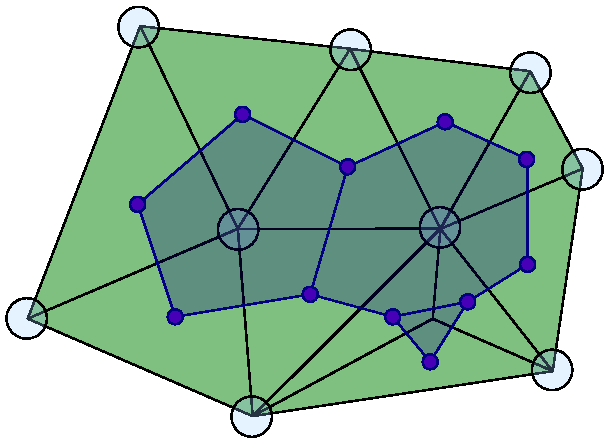
\includegraphics[height=3cm]{DualExample.pdf}
%\end{center}
%\caption{2D example of a dual mesh (blue) overlaid against a triangular mesh (green).}
%\label{fig:DualExample}
%\end{figure}

\subsection{Dual Mesh Generation Results}

\begin{figure}[!tb]
\begin{center}
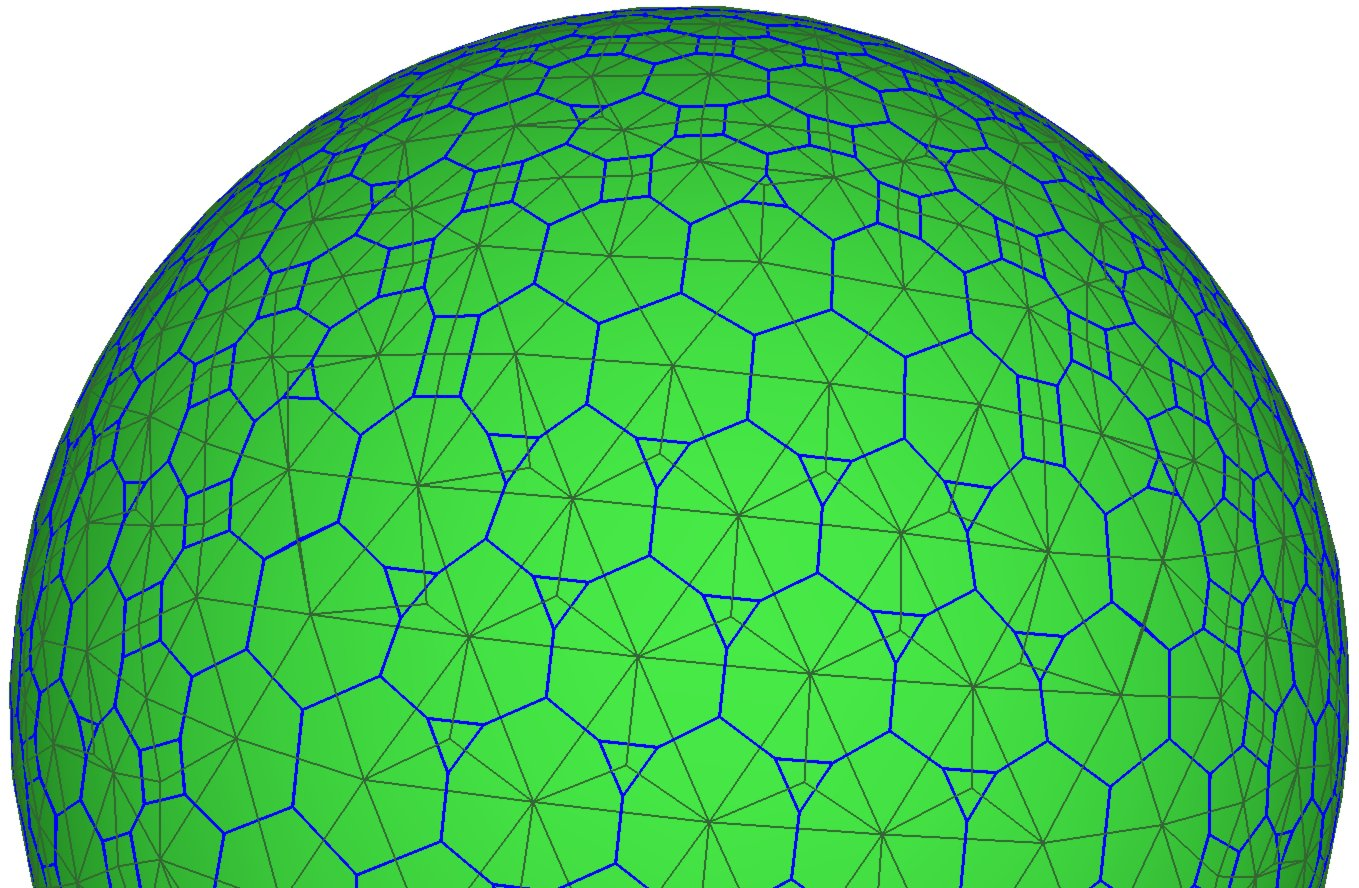
\includegraphics[width=\linewidth]{DualMeshSkeleton.jpg}
\end{center}
\caption{Dual mesh (blue) overlaid as as a skeleton upon a triangular contour mesh (green) that was generated by Marching Cubes with the spherical distance dataset.}
\label{fig:DualMeshSkeleton}
\end{figure}
Figure~\ref{fig:DualMeshSkeleton} shows a mesh and its dual overlaid as a skeleton. Table~\ref{tab:timingsdualmesh} shows the timings for generating dual meshes. Similarly to the case for local averaging, the time taken to generate a dual mesh is dominated by the time taken to remove unique elements from the incidence list, thereby generating an edge adjacency list. The time taken for generating a dual mesh exceeds that for the local averaging case because the face adjacency lists are larger than vertex incidence lists by a factor of 3. 

\begin{table}[tb!]
\begin{center}
\caption{Timings for dual mesh generation}
\label{tab:timingsdualmesh}
\begin{tabular}{l|r r r r|r r r}
\multicolumn{8}{c}{ } \\
 & \multicolumn{4}{|c|}{Spherical Distance} & \multicolumn{3}{|c}{MRI Head}\\
Arch. & $64^3$ & $128^3$ & $256^3$ & $512^3$ & $64^3$ & $128^3$ & $256^3$\\
\hline
CUDA & 20 & 64 & 255 & 1111 & 62 & 337 & 1480 \\
%OpenMP (1 thread) & 35 & 215 & 1410 & 6102 & 211 & 1383 & 5985 \\
OpenMP & 24 & 113 & 522 & 2263 & 115 & 531 & 2302
\end{tabular}
\end{center}
\vspace{-0.6cm}
\end{table}

\section{Conclusions and Future Work}
We provide an efficient, generalized method for parallel generation of topological connectivity information. We require little to no alteration to the algorithms generating geometry, although we leverage small modifications to allow for knowledge of input topological features for better performance. We demonstrate how to use such modifications to gain performance on structured grids, and to perform a simple mesh coarsening on either structured or unstructured grids. We demonstrate that our algorithm is effective on structured grids and on several different tetrahedral grids. 

Future work includes measurement of how well this technique can scale on architectures approaching the exascale and determining what bottlenecks, if any, need to be addressed for this transition. 

% needed in second column of first page if using \IEEEpubid
%\IEEEpubidadjcol


% An example of a floating figure using the graphicx package.
% Note that \label must occur AFTER (or within) \caption.
% For figures, \caption should occur after the \includegraphics.
% Note that IEEEtran v1.7 and later has special internal code that
% is designed to preserve the operation of \label within \caption
% even when the captionsoff option is in effect. However, because
% of issues like this, it may be the safest practice to put all your
% \label just after \caption rather than within \caption{}.
%
% Reminder: the "draftcls" or "draftclsnofoot", not "draft", class
% option should be used if it is desired that the figures are to be
% displayed while in draft mode.
%
%\begin{figure}[!t]
%\centering
%\includegraphics[width=2.5in]{myfigure}
% where an .eps filename suffix will be assumed under latex, 
% and a .pdf suffix will be assumed for pdflatex; or what has been declared
% via \DeclareGraphicsExtensions.
%\caption{Simulation Results}
%\label{fig_sim}
%\end{figure}

% Note that IEEE CS typically puts floats only at the top, even when this
% results in a large percentage of a column being occupied by floats.
% However, the Computer Society has been known to put floats at the bottom.


% An example of a double column floating figure using two subfigures.
% (The subfig.sty package must be loaded for this to work.)
% The subfigure \label commands are set within each subfloat command, the
% \label for the overall figure must come after \caption.
% \hfil must be used as a separator to get equal spacing.
% The subfigure.sty package works much the same way, except \subfigure is
% used instead of \subfloat.
%
%\begin{figure*}[!t]
%\centerline{\subfloat[Case I]\includegraphics[width=2.5in]{subfigcase1}%
%\label{fig_first_case}}
%\hfil
%\subfloat[Case II]{\includegraphics[width=2.5in]{subfigcase2}%
%\label{fig_second_case}}}
%\caption{Simulation results}
%\label{fig_sim}
%\end{figure*}
%
% Note that often IEEE CS papers with subfigures do not employ subfigure
% captions (using the optional argument to \subfloat), but instead will
% reference/describe all of them (a), (b), etc., within the main caption.


% An example of a floating table. Note that, for IEEE style tables, the 
% \caption command should come BEFORE the table. Table text will default to
% \footnotesize as IEEE normally uses this smaller font for tables.
% The \label must come after \caption as always.
%
%\begin{table}[!t]
%% increase table row spacing, adjust to taste
%\renewcommand{\arraystretch}{1.3}
% if using array.sty, it might be a good idea to tweak the value of
% \extrarowheight as needed to properly center the text within the cells
%\caption{An Example of a Table}
%\label{table_example}
%\centering
%% Some packages, such as MDW tools, offer better commands for making tables
%% than the plain LaTeX2e tabular which is used here.
%\begin{tabular}{|c||c|}
%\hline
%One & Two\\
%\hline
%Three & Four\\
%\hline
%\end{tabular}
%\end{table}


% Note that IEEE does not put floats in the very first column - or typically
% anywhere on the first page for that matter. Also, in-text middle ("here")
% positioning is not used. Most IEEE journals use top floats exclusively.
% However, Computer Society journals sometimes do use bottom floats - bear
% this in mind when choosing appropriate optional arguments for the
% figure/table environments.
% Note that, LaTeX2e, unlike IEEE journals, places footnotes above bottom
% floats. This can be corrected via the \fnbelowfloat command of the
% stfloats package.





% if have a single appendix:
%\appendix[Proof of the Zonklar Equations]
% or
%\appendix  % for no appendix heading
% do not use \section anymore after \appendix, only \section*
% is possibly needed

% use appendices with more than one appendix
% then use \section to start each appendix
% you must declare a \section before using any
% \subsection or using \label (\appendices by itself
% starts a section numbered zero.)
%


\appendices
%\section{Proof of the First Zonklar Equation}
%Appendix one text goes here.

% you can choose not to have a title for an appendix
% if you want by leaving the argument blank

% use section* for acknowledgement
\ifCLASSOPTIONcompsoc
  % The Computer Society usually uses the plural form
  \section*{Acknowledgments}
\else
  % regular IEEE prefers the singular form
  \section*{Acknowledgment}
\fi


This work was supported in full by the DOE Office of Science, Advanced Scientific Computing Research, under award number 10-014707, program manager Lucy Nowell.

Part of this work was performed by Sandia National Laboratories.  Sandia National Laboratories is a multi-program laboratory operated by Sandia Corporation, a wholly owned subsidiary of Lockheed Martin Corporation, for the U.S. Department of Energy's National Nuclear Security Administration.


% Can use something like this to put references on a page
% by themselves when using endfloat and the captionsoff option.
\ifCLASSOPTIONcaptionsoff
  \newpage
\fi



% trigger a \newpage just before the given reference
% number - used to balance the columns on the last page
% adjust value as needed - may need to be readjusted if
% the document is modified later
%\IEEEtriggeratref{8}
% The "triggered" command can be changed if desired:
%\IEEEtriggercmd{\enlargethispage{-5in}}

% references section

% can use a bibliography generated by BibTeX as a .bbl file
% BibTeX documentation can be easily obtained at:
% http://www.ctan.org/tex-archive/biblio/bibtex/contrib/doc/
% The IEEEtran BibTeX style support page is at:
% http://www.michaelshell.org/tex/ieeetran/bibtex/
\bibliographystyle{IEEEtran}
% argument is your BibTeX string definitions and bibliography database(s)
%%%%%%%\bibliography{IEEEabrv, ./TopologyReconstruction.bib}

\begin{thebibliography}{10}

\bibitem{Bank2003}
R.~E. Bank and M.~Holst.
\newblock {A New Paradigm for Parallel Adaptive Meshing Algorithms}.
\newblock {\em SIAM Review}, 45(2):291, 2003.

\bibitem{Bell2010}
N.~Bell.
\newblock {High-Productivity CUDA Development with the Thrust Template
  Library}, 2010.

\bibitem{Bell2012}
N.~Bell and J.~Hoberock.
\newblock {Thrust: A Productivity-Oriented Library for CUDA}.
\newblock {\em thrust.googlecode.com}, pages 359--373, 2012.

\bibitem{Blelloch1990}
G.~Blelloch.
\newblock {Prefix sums and their applications}.
\newblock {\em Synthesis of Parallel Algorithms}, pages 35--60, 1990.

\bibitem{Blelloch1991}
G.~E. Blelloch.
\newblock {Vector Models for Data-Parallel Computing}.
\newblock {\em Computing Control Engineering Journal}, 2(5):238, 1991.

\bibitem{Boubekeur2005}
T.~Boubekeur and C.~Schlick.
\newblock {Generic mesh refinement on GPU}.
\newblock In {\em Proceedings of the ACM SIGGRAPH/EUROGRAPHICS conference on
  graphics hardware}, number July, pages 99--104. ACM, 2005.

\bibitem{Carr2006}
H.~Carr, T.~M\"{o}ller, and J.~Snoeyink.
\newblock {Artifacts caused by simplicial subdivision.}
\newblock {\em IEEE transactions on visualization and computer graphics},
  12(2):231--42, 2006.

\bibitem{Computing1992}
H.~P. Computing.
\newblock {Scientific Visualization with VTK, The Visualization Toolkit}.
\newblock {\em Fluid Dynamics}, 12(1):1--9, 1992.

\bibitem{MapReduce}
J.~Dean and S.~Ghemawat.
\newblock {MapReduce}: Simplified data processing on large clusters.
\newblock {\em Communications of the ACM}, 51(1):107--113, January 2008.

\bibitem{DeCoro2007}
C.~DeCoro and N.~Tatarchuk.
\newblock Real-time mesh simplification using the {GPU}.
\newblock In {\em Proceedings of the 2007 Symposium on Interactive 3D Graphics
  and Games (I3D '07)}, pages 161--166, 2007.
\newblock {DOI}~10.1145/1230100.1230128.

\bibitem{Dyken2008}
C.~Dyken, G.~Ziegler, C.~Theobalt, and H.-P. Seidel.
\newblock {High-speed Marching Cubes using HistoPyramids}.
\newblock {\em Computer Graphics Forum}, 27(8):2028--2039, 2008.

\bibitem{Garland2001}
M.~Garland, A.~Willmott, and P.~S. Heckbert.
\newblock {Hierarchical face clustering on polygonal surfaces}.
\newblock {\em Proceedings of the 2001 symposium on Interactive 3D graphics
  SI3D 01}, pages 49--58, 2001.

\bibitem{Goetz_Junklewitz_Domik_2005}
F. Goetz, T. Junklewitz and G. Domik.
\newblock Real-Time Marching Cubes on the Vertex Shader.
\newblock In {\em EUROGRAPHICS}, pages 1--4, 2005.

\bibitem{Hoppe1996}
H.~Hoppe.
\newblock {Progressive meshes}.
\newblock {\em Proceedings of the 23rd annual conference on Computer graphics
  and interactive techniques SIGGRAPH 96}, 30(3):99--108, 1996.

\bibitem{Horn2005}
D.~Horn.
\newblock {Stream Reduction Operations for GPGPU Applications}.
\newblock In M.~Pharr, editor, {\em GPU Gems 2}, volume~2, chapter~36, pages
  573--589. Addison Wesley, 2005.

\bibitem{Hsieh2005}
H.~Hsieh and W.~Tai.
\newblock {A simple GPU-based approach for 3D Voronoi diagram construction and
  visualization}.
\newblock {\em Simulation Modelling Practice and Theory}, 13(8):681--692, Nov.
  2005.
  
\bibitem{Johansson_Carr_2006}
G. Johansson and H. Carr.
\newblock Accelerating marching cubes with graphics hardware.
\newblock In {\em Proceedings of the 2006 conference of the Center for Advanced Studies on Collaborative research CASCON 06}, page 39, 2006.

\bibitem{Kipfer2005}
P.~Kipfer and R.~Westermann.
\newblock {GPU construction and transparent rendering of iso-surfaces}.
\newblock In {\em Proceedings Vision, Modeling and Visualization}, volume~5,
  2005.

\bibitem{Lindstrom2000}
P.~Lindstrom.
\newblock {Out-of-core simplification of large polygonal models}.
\newblock In {\em Proceedings of the 27th annual conference on Computer
  graphics and interactive techniques}, pages 259--262. ACM
  Press/Addison-Wesley Publishing Co., 2000.

\bibitem{Lorensen1987}
W.~E. Lorensen and H.~E. Cline.
\newblock {Marching cubes: A high resolution 3D surface construction
  algorithm}.
\newblock {\em Computer}, 21(4):163--169, 1987.

\bibitem{Moore_Warren_1991}
D. Moore and J. D. Warren.
\newblock Mesh displacement: An improved contouring method for trivariate data.
\newblock In {\em Computer}, pages 1--15, 1991

\bibitem{Park}
J.~Park, B.~Choi, and Y.~Chung.
\newblock {Efficient topology construction from triangle soup}.
\newblock In {\em Geometric Modeling and Processing, Proceedings}, volume~1,
  pages 359--364. IEEE, 2004.

\bibitem{Potter2011}
M.~Potter.
\newblock {\em Anisotropic mesh coarsening and refinement on {GPU}
  architecture}.
\newblock PhD thesis, Imperial College London, Department of Computing, June
  2011.

\bibitem{Rottger2000}
S.~R\"{o}ttger, M.~Kraus, and T.~Ertl.
\newblock {Hardware-accelerated volume and isosurface rendering based on
  cell-projection}.
\newblock In {\em Proceedings of the conference on Visualization'00}, pages
  109--116. IEEE Computer Society Press, 2000.

\bibitem{Sengupta2007}
S.~Sengupta, M.~Harris, Y.~Zhang, and J.~D. Owens.
\newblock {Scan Primitives for GPU Computing}.
\newblock {\em Computing}, 21(3):106, 2007.

\bibitem{Sifakis2007}
E.~Sifakis.
\newblock {Arbitrary Cutting of Deformable Tetrahedralized Objects}.
\newblock {\em Computing}, 1, 2007.

\bibitem{Stuart2010}
J.~A. Stuart, C.-K. Chen, K.-L. Ma, and J.~D. Owens.
\newblock Multi-{GPU} volume rendering using {MapReduce}.
\newblock In {\em 1st International Workshop on MapReduce and its
  Applications}, June 2010.

\bibitem{Vo2011}
H.~T. Vo, J.~Bronson, B.~Summa, J.~L. Comba, J.~Freire, B.~Howe, V.~Pascucci,
  and C.~T. Silva.
\newblock Parallel visualization on large clusters using {MapReduce}.
\newblock In {\em Proceedings of the IEEE Symposium on Large-Scale Data
  Analysis and Visualization}, pages 81--88, October 2011.
\newblock {DOI}~10.1109/LDAV.2011.6092321.

\bibitem{Zhou_Hou_Wang_Guo_2008}
K. Zhou, Q. Hou, R. Wang, and B. Guo.
\newblock Real-time KD-tree construction on graphics hardware.
\newblock In {\em ACM Transactions on Graphics}, 27(5):1, 2008.

\end{thebibliography}

%
% <OR> manually copy in the resultant .bbl file
% set second argument of \begin to the number of references
% (used to reserve space for the reference number labels box)
%\begin{thebibliography}{1}

%\bibitem{IEEEhowto:kopka}
%This is an example of a book reference
%H. Kopka and P.W. Daly, \emph{A Guide to {\LaTeX}}, third ed. Harlow, U.K.: Addison-Wesley, 1999.


%This is an example of a Transactions article reference
%D.S. Coming and O.G. Staadt, "Velocity-Aligned Discrete Oriented Polytopes for Dynamic Collision Detection," IEEE Trans. Visualization and Computer Graphics, vol. 14,  no. 1,  pp. 1-12,  Jan/Feb  2008, doi:10.1109/TVCG.2007.70405.

%This is an example of a article from a conference proceeding
%H. Goto, Y. Hasegawa, and M. Tanaka, "Efficient Scheduling Focusing on the Duality of MPL Representation," Proc. IEEE Symp. Computational Intelligence in Scheduling (SCIS '07), pp. 57-64, Apr. 2007, doi:10.1109/SCIS.2007.367670.

%This is an example of a PrePrint reference
%J.M.P. Martinez, R.B. Llavori, M.J.A. Cabo, and T.B. Pedersen, "Integrating Data Warehouses with Web Data: A Survey," IEEE Trans. Knowledge and Data Eng., preprint, 21 Dec. 2007, doi:10.1109/TKDE.2007.190746.

%Again, see the IEEEtrans_HOWTO.pdf for several more bibliographical examples. Also, more style examples
%can be seen at http://www.computer.org/author/style/transref.htm
%\end{thebibliography}

% biography section
% 
% If you have an EPS/PDF photo (graphicx package needed) extra braces are
% needed around the contents of the optional argument to biography to prevent
% the LaTeX parser from getting confused when it sees the complicated
% \includegraphics command within an optional argument. (You could create
% your own custom macro containing the \includegraphics command to make things
% simpler here.)
%\begin{biography}[{\includegraphics[width=1in,height=1.25in,clip,keepaspectratio]{mshell}}]{Michael Shell}
% or if you just want to reserve a space for a photo:

%\begin{IEEEbiography}{Michael Shell}
%Biography text here.
%\end{IEEEbiography}

% if you will not have a photo at all:
%\begin{IEEEbiographynophoto}{John Doe}
%Biography text here.Biography text here.Biography text here.Biography text here.Biography text here.Biography text here.Biography text here.Biography text here.Biography text here.Biography text here.Biography text here.Biography text here.Biography text here.Biography text here.Biography text here.Biography text here.Biography text here.Biography text here.Biography text here.Biography text here.Biography text here.Biography text here.Biography text here.Biography text here.Biography text here.Biography text here.Biography text here.Biography text here.Biography text here.Biography text here.Biography text here.Biography text here.
%\end{IEEEbiographynophoto}

% insert where needed to balance the two columns on the last page with
% biographies
%\newpage

%\begin{IEEEbiographynophoto}{Jane Doe}
%Biography text here.Biography text here.Biography text here.Biography text here.Biography text here.Biography text here.Biography text here.Biography text here.Biography text here.Biography text here.Biography text here.Biography text here.Biography text here.Biography text here.Biography text here.Biography text here.Biography text here.Biography text here.Biography text here.Biography text here.Biography text here.Biography text here.Biography text here.Biography text here.Biography text here.Biography text here.Biography text here.Biography text here.
%\end{IEEEbiographynophoto}

% You can push biographies down or up by placing
% a \vfill before or after them. The appropriate
% use of \vfill depends on what kind of text is
% on the last page and whether or not the columns
% are being equalized.

%\vfill

% Can be used to pull up biographies so that the bottom of the last one
% is flush with the other column.
%\enlargethispage{-5in}



% that's all folks
\end{document}



